%%%%%%%%%%%%%%%%%%%%%%%%%%%%%%%%%%%%%%%%%%%%%%%%%%%%%%%%%%%%%%%%%%%%%%%%%%%%%%%%
%                                                                              %
%   PAW   - Reference Manual -- LaTeX Source                                   %
%                                                                              %
%   Chapter 3 : PAW Examples                                                   %
%                                                                              %
%   EPS file      : pawtut60b.eps                                              %
%                   example.eps                                                %
%                                                                              %
%   Editor: Michel Goossens / IT-ASD                                           %
%   Last Mod.: 30 July 1998 Olivier Couet                                      %
%                                                                              %
%%%%%%%%%%%%%%%%%%%%%%%%%%%%%%%%%%%%%%%%%%%%%%%%%%%%%%%%%%%%%%%%%%%%%%%%%%%%%%%%
\chapter{PAW by Examples}
\minitoc
\newpage
\section{Basic Principles}
\begin{itemize}
\item \PAW\ (Physics Analysis Workstation) is an {\em interactive system}
       designed for data analysis and data presentation.
\item \PAW\ provides a set of {\em commands} acting on specific objects. The
      main objects or data type are: {\em vectors}, {\em histograms}, and 
      {\em ntuples}. The aim of the examples is to explain how to work with 
      these objects.
\item The \PAW\ commands are organized in a {\em tree}, whose
      general structure is: \texttt{OBJECT/ACTION}. \\
Examples: \Ucom{NTUPLE/PLOT}, \Ucom{HISTOGRAM/PROJECT}, \Ucom{VECTOR/DRAW}
\item The usual user interface is a ``command line interface'': commands are
      typed on keyboard and executed after {\tt <CR>}. Commands parameters
      are separated with blank.
\item Command editing and retrieving is also possible. It is controlled
      via the command {\tt RECALL\_STYLE}.
\item Commands can be grouped into ``Macros''. Macros are files with the
      extension {\tt .kumac} containing \PAW\ commands and flow control
      operators like ``do loop'', ``if endif'', etc .. . To execute
      a macro it is enough to type {\tt EXEC macroname}.
\item online help can be obtained with the commands:
\begin{itemize}
   \item {\tt HELP} to have the full description of a command.
   \item {\tt USAGE} to have only the command syntax.
\end{itemize}
\item A printable version of the reference manual can be obtained with the
      command {\tt MANUAL}.
\item \PAW++ provides a Motif based User Interface to \PAW.
\item \PAW\ and \PAW++ have the SAME basic functionality.
\end{itemize}
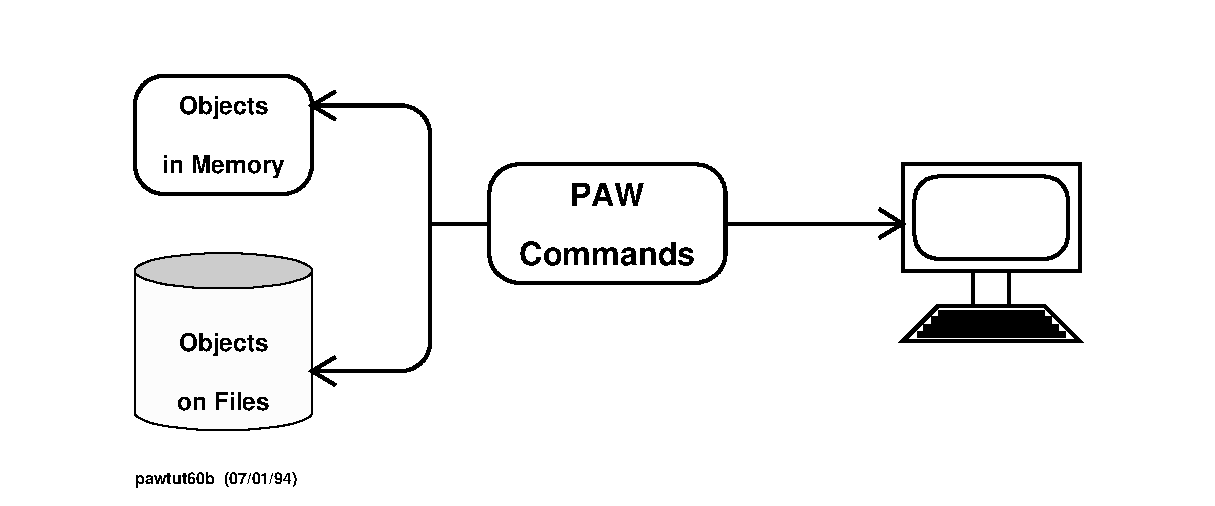
\epsfig{file=pawtut60b.eps,width=\linewidth}
\clearpage

\section{Starting the PAW Tutorial}
This tutorial present the basic principles of \PAW\ using a set of examples
(\PAW\ macros). It tries to cover the most frequently used basic functions of
\PAW.  
In the examples, highlighted points are written in UPPERCASE with a reference
in the left margin. This reference point to a comment after the listing
of the macro. If the example produce a graphics output, it is given on
the page behind the example. Under each figure, the name of the 
corresponding macro is given.

\begin{alltt}
      MACRO PAWLOGON
      Mess '*************************************************************'
      Mess '*                                                           *'
      Mess '*                  Starting PAW examples                    *'
      Mess '*                                                           *'
      Mess '*                     29-30 June 1993                       *'
      Mess '*                                                           *'
      Mess '*************************************************************'
\end{alltt}

This example shows what could be the {\tt MACRO PAWLOGON} (in the file
{\tt PAWLOGON.KUMAC}) which is automatically executed (if it exists) at the
beginning of each \PAW\ session.

It is assumed that the macro {\tt ALDDEF} is executed before each example.

\index{alldef.kumac}
\subsection*{alldef.kumac}
\begin{alltt}
      MACRO ALLDEF
      Size 18 24
      Next
      Set * ; Option * ; Igset *
      Size 18 24
      Histogram/Delete * ; Vector/Delete *
      Title_global ' '
      Title_global ' ' U
      Option NBOX
      Option NGRI
      Set *WID 1
      Set CSIZ 0.25 ; Set VSIZ 0.25 ; Set TSIZ 0.32
      Set XMGL 1.2  ; Set XMGR 1.2  ; Set YMGU 0.5 ; Set YMGL 1.5
      Set GSIZ 0.1
      Set YHTI 0.7
      Set KSIZ 0.15
      Set MTYP 1
      Zone 1 1
      Next
      Return
\end{alltt} 

%%%%%%%%%%%%%%%%%%%%%%%%%%%%%%%%%%%%%%%%%%%%%%%%%%%%%%%%%%%%%%%%%%%%%%%%%%%%%%%%
\clearpage
\section{Vectors---Tutorial}
\label{sec:tutvectors}
\pawtutfig{20}
\clearpage
\pawtutfig{21}
\clearpage
\pawtutfig{28}
\clearpage
\pawtutfig{29}
\clearpage
\section{Vectors---Examples}
\subsection{Starting with vectors}
\begin{alltt}
\Bn{6}     * Starting with vectors
\Bn{6}     VECTOR/CREATE VECT1(10)  | Create a vector of length 10
\Bn{1}     VECTOR/INPUT VECT1 10 8 6 4 2 3 5 7 9 11
\Bnii{7}{1}   VECTOR/CRE VX(20) R 1. 2. 3. 4. 5. 6. 7. 8. 9. _
      10. 11. 12. 13. 14. 15. 16. 17. 18. 19. 20.
      v/cr vy(20) r 1.1 3.2 5.3 7.4 7.5 6.6 4.3 2.1 6.6 _
      11.1 16.2 18.3 19.0 17.8 16.0 12.1 9.1 6.1 3.1 6.6
\Bn{8}     ZON 1 2
\Bn{2}     VECTOR/DRAW VECT1
\Bnii{4}{2}   GRAPH 20 VX VY
\Bnii{4}{5}   graph 20 VX VY *
\Bn{5}     gra 20 VX VY C
\Bn{3}     VECT/DEL *
\end{alltt} 
\begin{DinglistE}
\item Here we see two ways to fill a vector:
\begin{enumerate}
   \item {\tt V/CREATE}: create a vector and, optionally, fill it.
         \index{vector!create}
   \item {\tt V/INPUT}: allows to fill an existing vector.
         \index{vector!input}
\end{enumerate}
We will see other ways later.
\item Graphic representations of vectors : {\tt VECTOR/DRAW} and
      {\tt GRAPH}. \index{vector!draw} \index{vector!graph}
\item {\tt VECT/DELETE} allows to delete a vector from memory. ``*'' means
      delete all vectors in memory. Very often in \PAW\ a command acting
      on a specific kind of objects (vectors, histogram, pictures) can
      access the complete object set with ``*''. \index{vector!delete}

\underline{Note also:}

\item The \PAW\ commands are case insensitive.
\item Command abbreviations are permitted.
\item The character ``*'' and ``$\mid$'' are used for comments.
\item The character ``\_'' is used to indicate a continuation line.
\item The command {\tt ZONE} subdivides the graphical area.
\end{DinglistE}
\pawexfig{1}

%%%%%%%%%%%%%%%%%%%%%%%%%%%%%%%%%%%%%%%%%%%%%%%%%%%%%%%%%%%%%%%%%%%%%%%%%%%%%%%%
\clearpage

\subsection{Some more vector commands}
\begin{alltt}
      vector/create VECT(10,3) R _
      1. 2. 3. 4. 5. 6. 7. 8. 9. 10. _
      9.1 8.1 7.1 6.1 5.1 4.1 3.1 2.1 1.1 0.1 _
      6.2 4.2 3.2 2.2 1.2 1.2 2.2 3.2 4.2 5.2
      vector/create VECT1(10) R _
      1.1 2.2 3.3 4.4 5.5 6.6 5.5 4.4 3.3 2.2
\Bn{5}     SET HTYP 244 ; VE/DR VECT(1:10,3)
\Bnii{1}{2}   VECTOR/DRAW VECT(1:10,3) ! SC
\Bnii{4}{6}   VECTOR/DRAW VECT1 ! L*S
      ve/list
\Bn{3}     VE/WRITE VECT 'vector.data' '(3(10f5.0,/))'
\end{alltt} 
\begin{DinglistE}
\index{vector!draw}
\index{vector!dimensions}
\item A vector can have up to three dimensions. Dimensions which are not
      specified are taken as 1, for example {\tt VEC(10) $\rightarrow$
      VEC(10,1,1)} and {\tt VEC $\rightarrow$ VEC(1,1,1)}.
      \index{vector!subranges}
\item It is possible to access a subrange of a vector, for example:
      {\tt V(2:3)}, {\tt V(3:)} or {\tt V(:5)}. \index{vector!write}
\item The command {\tt VECT/WRITE} creates the file {\tt vector.data}
      as follows:
\begin{verbatim}
     1.   2.   3.   4.   5.   6.   7.   8.   9.  10.
     9.   8.   7.   6.   5.   4.   3.   2.   1.   0.
     6.   4.   3.   2.   1.   1.   2.   3.   4.   5.
\end{verbatim}

\underline{Note also:}

\item The character ``!'' means default value of a parameter.
\item It is possible to have several commands, separated with ``;'', on
      the same line.
\item Many commands have a parameter which defines
      options. Such parameters (often called {\tt CHOPT} or {\tt OPTION})
      have the attribute ``Option'' (see the help). Each option is 
      a character string. It is possible to mix several options, e.g.
      ``{\tt SC}'' or ``{\tt L*S}''.
\end{DinglistE}

\pawexfig{2}

%%%%%%%%%%%%%%%%%%%%%%%%%%%%%%%%%%%%%%%%%%%%%%%%%%%%%%%%%%%%%%%%%%%%%%%%%%%%%%%%
\clearpage

\subsection{Possible data representations with VECTOR/DRAW}
\begin{alltt}
      zone 2 3
      ve/create v(10) R 5 1 3 2 4 1 3 1 8 6
\Bn{1}     SET HTYP 244
      ve/draw v
      ve/draw v ! b
      ve/draw v ! l
\Bn{3}     VE/DRAW V CHOPT=L*
      ve/draw v ! bl*
\Bn{2}     IGSET MTYP 21
      ve/draw v ! e
      ve/de V
\Bn{4}     RETURN
\end{alltt} 
\begin{DinglistE}
\index{vector!draw}
\item The command {\tt SET} defines some high level
      graphics attributes for commands like {\tt VECT/DRAW} or {\tt HIST/PLOT}.
      Here the {\tt HTYP} (Histogram hatch TYPe) is defined.
      \index{IGSET} \index{SET}
\item {\tt IGSET} is used to define basic graphics
      attributes like line width, marker type etc ... . Here the marker
      type is defined. It is possible to type always {\tt SET} instead 
      of {\tt IGSET} i.e. if a {\tt IGSET} parameter is invoke with the
      {\tt SET} command, the command {\tt IGSET} is automatically invoked.
      \index{command!parameter}
\item By default the parameters of a command are positional but it is
      possible to assign values by name, i.e. {\tt PARAMETER=value}. For
      example we have here {\tt CHOPT=L*}. In this case the ``!'' can be
      suppressed.

\underline{Note also:}

\item The statement {\tt RETURN} is not mandatory in a macro except if there
      are several macros in the same file. In this case, a macro within a
      file can be executed by: {\tt EXEC FILENAME\#MACRONAME}.
      \index{\texttt{RETURN}}
\end{DinglistE}
\pawexfig{3}

%%%%%%%%%%%%%%%%%%%%%%%%%%%%%%%%%%%%%%%%%%%%%%%%%%%%%%%%%%%%%%%%%%%%%%%%%%%%%%%%
\clearpage

\subsection{Vectors and Histograms}
\label{sec:vectordrawplot}
\subsection*{Functionality of VECT/DRAW, VECT/PLOT, VECT/HFILL and
  PUT/CONT}
\begin{alltt}
      zone 2 2
      ve/create VECT1(10) R 1 2 3 4 5 5 4 3 2 1
      *
      ve/draw VECT1
\Bn{1}     VE/PLOT VECT1
      *
\Bn{4}     CREATE/1DHISTO 100 'test vector/hfill' 5 1. 6.
      max 100 2.5
\Bn{2}     VE/HFILL VECT1 100
      histo/plot 100 b
      hi/de 100
      *
      create/1dhisto 100 'test put/contents' 10 1. 11.
\Bn{5}     MAX 100 5.5
\Bn{5}     MIN 100 0.5
\Bn{3}     PUT/CONTENTS 100 VECT1
      histo/plot 100
\end{alltt} 
\index{vector!draw}
\index{vector!plot}
\index{vector!hfill}
\index{put!contents}
\begin{DinglistE}
\item {\tt VECT/PLOT} draws the statistic of the given vector.
\item {\tt VECT/HFILL} fills an existing histogram (create with
      {\tt 1DHIST}) with the values taken from a vector. Note that the
      command {\tt VECTOR/PLOT} can automatically book an histogram
      and fill it with the vector content.
\item {\tt PUT/CONT} replaces the content of an histogram with
     the values of a vector.

\underline{Note also:}

\item Histograms are \HBOOK\ objects. They can be created, like here,
      interactively in \PAW\ or in a batch \HBOOK\ program.They can be 
      stored in direct access files (we will see examples later).
\index{histogram!minimum}
\index{histogram!maximum}
\item {\tt MIN} and {\tt MAX} define the minimum and maximum of
      an histogram. By default they are computed automatically.
\end{DinglistE}
\pawexfig{4}

%%%%%%%%%%%%%%%%%%%%%%%%%%%%%%%%%%%%%%%%%%%%%%%%%%%%%%%%%%%%%%%%%%%%%%%%%%%%%%%%
\clearpage

\subsection{Vector operations}
\index{vector!operations}
\begin{alltt}
      zone 1 2
      ve/create V1(10) R 1 2 3 4 5 5 4 3 2 1
      vector/operations/vscale V1 0.5   V12
\Bn{1}     VE/OP/VSCALE             V1 0.25  V14
      ve/dr V1
      ve/dr V12 ! S
      ve/dr V14 ! S
\Bn{1}     VSUB                      V1 V14 V14M
      ve/dr V1
      set htyp 344
      ve/dr V14M ! S
      set htyp 144
      ve/dr V12  ! S
\end{alltt} 
\begin{DinglistE}
\item Some simple operations are possible on vectors:
\begin{verbatim}
      VBIAS     : Y(i) = a + X(i)
      VSCALE    : Y(i) = a * X(i)
      VADD      : Z(i) = X(i) + Y(i)
      VMULTIPLY : Z(i) = Z(i) * Y(i)
      VSUBSTRACT: Z(i) = X(i) - Y(i)
      VDIVIDE   : Z(i) = X(i) / Y(i)
\end{verbatim}
  In these operations the resulting vectors are created automatically.
  Note that for more complicate operations like {\tt SQRT} or trigonometric
  functions etc... , \SIGMA\ must be used (we will see examples later).
\end{DinglistE}
\pawexfig{5}

%%%%%%%%%%%%%%%%%%%%%%%%%%%%%%%%%%%%%%%%%%%%%%%%%%%%%%%%%%%%%%%%%%%%%%%%%%%%%%%%
\clearpage

\subsection{Simple macro, with a loop and a VECTOR fit}

\begin{alltt}
      ve/create VECT(10,3)
\Bn{1}     VE/READ VECT 'vector.data'
      *
      ve/print VECT(1:10,3)
      vbias vect(1:10,1) 0.5 vect(1:10,1)
      zon 1 2
      *
\Bn{4}     DO IP = 2,3
        ve/draw vect(1:10,[ip])
\Bnii{2}{3}     ORDER = [IP] - 1
\Bn{5}       VECT/FIT VECT(1:10,1) VECT(1:10,[IP]) ! P[order] WS
\Bn{4}     ENDDO
      ve/delete VECT
\end{alltt} 
\begin{DinglistE}
\item The file {\tt vector.data} previously created is read again in
      this example via the command {\tt VECT/READ}. Note that it
      is not necessary to specify the format. \index{vector!read}
\item This example shows the usage of variables in the macros ({\tt IP}).
      The content of a variable can be accessed via:
\index{macro!variable}
\index{macro!loop}
\begin{verbatim}
                      [variable]
\end{verbatim}
      Note that the name of a variable in not case sensitive.
\item Simple computations on variables are possible, like {\tt i=[i]+1}
      or {\tt a=[b]+2}. However it is not possible to do complex operations
      on variables. For this kind of computation vectors and \SIGMA\
      (or \COMIS) must be used.
\item Some controls statements are available in macros (see the complete
      list in the next example).
\item It is possible to fit the vectors with functions. Here the
      function used for the fit is a polynome. The fitting mechanisms are very
      complete in \PAW\ and simple to use. All the details useful to use the
      commands {\tt HIST/FIT} and {\tt VECT/FIT} are given in the \PAW\ manual.
\end{DinglistE}
\pawexfig{6}

%%%%%%%%%%%%%%%%%%%%%%%%%%%%%%%%%%%%%%%%%%%%%%%%%%%%%%%%%%%%%%%%%%%%%%%%%%%%%%%%
\clearpage

\subsection{Macros flow control}

There are several constructs available for controlling the flow execution,
which include conditional statement blocks, several looping constructs and
variable assignation.

\index{macro!flow control}
\begin{center}
\begin{tabular}{|l|l|} \hline
\multicolumn{2}{|c|}{\bf Macro Statements} \\ \hline
{\sc Statement}                         & {\sc Description} \\
\hline
{\tt MACRO mname par1=val1 ...}         & begin macro {\tt mname} \\
{\tt EXEC mname par1 par2=val2 ...}     & execute macro {\tt mname} \\
{\tt RETURN}                            & end of a macro \\
{\tt READ par}                 & read macro parameter {\tt par} from keyboard \\
{\tt SHIFT}                             & control parameters list \\
{\tt label:}                            & label (must terminate with a colon) \\
{\tt GOTO label}                        & jump to {\tt label} \\
{\tt ON ERROR GOTO label}  & resume at {\tt label} on error condition \\
{\tt OF ERROR}    & temporarily deactivate the {\tt ON ERROR GOTO} handling   \\
{\tt ON ERROR}    & reactivate the latest {\tt ON ERROR GOTO} handling        \\
{\tt IF logical\_expression GOTO label} & conditional statement \\
{\tt IF-THEN, ELSEIF, ELSE, ENDIF}      & Macro flow control    \\
{\tt CASE, ENDCASE}                     & Macro flow control    \\
{\tt WHILE-DO, ENDWHILE}                & Macro flow control    \\
{\tt REPEAT, UNTIL}                     & Macro flow control    \\
{\tt DO, ENDDO}                         & Macro flow control    \\
{\tt FOR, ENDFOR}                       & Macro flow control    \\
{\tt BREAKL}                            & Macro flow control    \\
{\tt EXITM}                             & Macro termination     \\
par = arithmetic\_expression            & assignment statement  \\
\hline
\end{tabular}
\end{center}

\index{macro!conditional statement}
\subsection*{Conditional statement}
\begin{alltt}
 MACRO DOC1                                        PAW > EXEC DOC1
   A = 10                                          Sum of 10 and 1.5 is 11.5
   NN = 1.5                                        KUIP arithmetic is correct.
   TOT = [A]+[NN]
   IF [TOT] > 11 THEN
     MESSAGE Sum of [A] and [NN] is [TOT]
     AOK = correct
   ELSE
     AOK = wrong
   ENDIF
   MESSAGE KUIP arithmetic is [AOK].
 RETURN
\end{alltt}

\clearpage
\subsection*{Unassigned variables cannot be substituted by their
  values.}
\begin{alltt}
 MACRO DOC2                                        PAW > EXEC DOC2
    A = 10                                         Result of sum is 10+[XX]
    NN = 1.5
    TOT = [A]+[XX]
    MESSAGE Result of sum is [TOT]
 RETURN
\end{alltt}

%%%%%%%%%%%%%%%%%%%%%%%%%%%%%%%%%%%%%%%%%%%%%%%%%%%%%%%%%%%%%%%%%%%%%%%%%%%%%%%%
\clearpage

\subsection{More on fits}
\subsection*{Fit the sine function sin between 0 and $2\pi$}
\begin{alltt}
\Bn{4}     APPLICATION SIGMA
\Bn{4}        alpha=array(100,0#2*PI)
\Bn{4}        sina=sin(alpha)+rndm(alpha)*0.1
\Bn{4}        err=array(100,0.1#0.1)
\Bn{4}     EXIT
      zone 2 2
\Bn{1}     V/FIT ALPHA(1:50) SINA(1:50) ERR(1:50) G
\Bn{1}     V/FIT ALPHA SINA ERR P3
\Bn{1}     V/FIT ALPHA SINA ERR P5
      v/create par(1) r 10.
\Bn{2}     V/FIT ALPHA SINA ERR SINFIT.F ! 1 PAR
\Bn{3}     V/PRI PAR
\end{alltt} 
\begin{DinglistE}
\item In this macro two different types of predefined fits are used: Gaussian,
      Polynomial. As we will see later, the histograms fitting command
      {\tt HISTO/FIT} has exactly the same syntax except that the 3 vectors
      are replaced by an unique parameter: The histogram identifier.
      On histograms some other minimization mechanisms are available via
      the commands {\tt SPLINE}, {\tt SMOOTH}, etc.. .
      \index{vector!fit}
\item It is also possible to defined specific functions. Here the function
      {\tt SINFIT} is defined as follow:
\subsection*{The function {\tt SINFIT}}
\begin{alltt}
      function sinfit(x)
      common /pawpar/ par(1)
      sinfit=par(1)*sin(x)
      end
\end{alltt} 
\item This {\tt VECT/PRI} shows that now {\tt PAR(1)} is close to 1.
\begin{verbatim}
      PAR(1) = 0.994221
\end{verbatim}
\item Vector initialization with \SIGMA. We will see other \SIGMA\ examples
      later.
\end{DinglistE}
\pawexfig{6c}
\clearpage
\subsection*{Output of the Gaussian fit}
\begin{alltt}
     **********************************************
     *                                            *
     * Function minimization by SUBROUTINE HFITV  *
     * Variable-metric method                     *
     * ID =          0  CHOPT =                   *
     *                                            *
     **********************************************
 Convergence when estimated distance to minimum (EDM) .LT.   .10E-03

 FCN=   2221.676     FROM MIGRAD    STATUS=CONVERGED    239 CALLS      240 TOTAL

                     EDM=   .85E-05    STRATEGY= 1      ERROR MATRIX ACCURATE

  EXT PARAMETER                                   STEP         FIRST
  NO.   NAME        VALUE          ERROR          SIZE      DERIVATIVE
   1      P1        1.1316        .24808E-01    .64412E-03    .15289
   2      P2        1.5419        .21417E-01    .62018E-03    .42301E-01
   3      P3       -.76813        .17032E-01    .43531E-03   -.25527
\end{alltt}
\subsection*{Output of the Polynomial fit (P3)}
\begin{alltt}
 CHISQUARE =  .2290E+02  NPFIT =  100
     **********************************************
     *                                            *
     * Function minimization by SUBROUTINE HFITV  *
     * Variable-metric method                     *
     * ID =          0  CHOPT =                   *
     *                                            *
     **********************************************
 Convergence when estimated distance to minimum (EDM) .LT.   .10E-03

 FCN=   49.31862     FROM MIGRAD    STATUS=FAILED        90 CALLS       91 TOTAL
                     EDM=   .79E-01  STRATEGY=1  ERROR MATRIX UNCERTAINTY= 70.2%

  EXT PARAMETER                APPROXIMATE        STEP         FIRST
  NO.   NAME        VALUE          ERROR          SIZE      DERIVATIVE
   1      P1       -.13523        .34965E-02    .00000E+00    5.6896
   2      P2        1.8729        .53793E-02    .00000E+00   -6.8643
   3      P3       -.86391        .32623E-03    .00000E+00    94.054
   4      P4        .91424E-01    .23105E-03    .00000E+00    6.6564

 CHISQUARE =  .5137E+00  NPFIT =  100
\end{alltt}
\clearpage
\subsection*{Output of the Polynomial fit (P5)}
\begin{alltt}
     **********************************************
     *                                            *
     * Function minimization by SUBROUTINE HFITV  *
     * Variable-metric method                     *
     * ID =          0  CHOPT =                   *
     *                                            *
     **********************************************
 Convergence when estimated distance to minimum (EDM) .LT.   .10E-03

 FCN=   7.164283     FROM MIGRAD    STATUS=FAILED       240 CALLS      241 TOTAL
                     EDM=   .19E+01    STRATEGY= 1      ERR MATRIX NOT POS-DEF

  EXT PARAMETER                APPROXIMATE        STEP         FIRST
  NO.   NAME        VALUE          ERROR          SIZE      DERIVATIVE
   1      P1        .46785E-01    .20704E-03    .68172E-07    32.993
   2      P2        .93224        .10038E-02    .74579E-06   -551.05
   3      P3        .20962        .33827E-03    .16770E-06   -3073.1
   4      P4       -.36899        .32674E-03    .29519E-06   -1084.4
   5      P5        .82836E-01    .19712E-04    .66269E-07    821.80
   6      P6       -.52834E-02    .12561E-05    .42267E-08   -5204.8

 CHISQUARE =  .7622E-01  NPFIT =  100
\end{alltt}
\subsection*{Output of the ``\COMIS'' fit}
\begin{alltt}
     **********************************************
     *                                            *
     * Function minimization by SUBROUTINE HFITV  *
     * Variable-metric method                     *
     * ID =          0  CHOPT =                   *
     *                                            *
     **********************************************
 Convergence when estimated distance to minimum (EDM) .LT.   .10E-03

 FCN=   32.13273     FROM MIGRAD    STATUS=CONVERGED     21 CALLS       22 TOTAL
                     EDM=   .92E-05    STRATEGY= 1      ERROR MATRIX ACCURATE

  EXT PARAMETER                                   STEP         FIRST
  NO.   NAME        VALUE          ERROR          SIZE      DERIVATIVE
   1      P1        .99811        .13752E-01    .51510E-04   -.31172

 CHISQUARE =  .3246E+00  NPFIT =  100
\end{alltt}

%%%%%%%%%%%%%%%%%%%%%%%%%%%%%%%%%%%%%%%%%%%%%%%%%%%%%%%%%%%%%%%%%%%%%%%%%%%%%%%%
\clearpage

\subsection{VECTOR/READ using MATCH}
\index{vector!read!using match}
\index{match}
\begin{alltt}
\Bn{1}     V/READ X,Y,Z match.dat 6x,3(F4.1) ! /Data/
      v/draw X
      v/draw Y ! S
      v/draw Z ! S
\end{alltt} 
\subsection*{match.dat}
\begin{alltt}
\Bn{2}     Title: File used for tests of the MATCH parameter in V/READ
      Data : 1.0 2.0 3.0
      Data : 2.0 3.0 4.0
      Data : 3.0 4.0 5.0
      Data : 4.0 5.0 6.0
\Bn{2}     This line will be ignored by a V/READ with MATCH
      Data : 5.0 6.0 7.0
      Data : 6.0 7.0 8.0
      Data : 7.0 8.0 9.0
      Data : 8.0 9.0 1.0
      Data : 9.0 1.0 2.0
\Bn{2}     End
\end{alltt} 
This example shows how the {\tt MATCH} parameter can be used in order to
read only a subset of a file. {\tt MATCH} is used to specify a pattern 
string, restricting the vector filling only to the records in the file 
which verify the pattern. Example of patterns: 
\begin{itemize}
\item     /string/      match a string (starting in column 1)
\item    -/string/      do not match a string (starting in column 1)
\item     /string/(n)   match a string, starting in column n
\item     /string/(*)   match a string, starting at any column
\end{itemize}
\begin{DinglistE}
\item When the {\tt MATCH} parameter is used, the command {\tt V/READ} reads
      the file in two passes:
\begin{enumerate}
\item to find how many lines should be read in order to create vectors with
      the proper length.
\item to read the lines where the {\tt MATCH} parameter is found.
\end{enumerate}
\item these lines are skipped during the reading pass.
\end{DinglistE}
\pawexfig{6d}

%%%%%%%%%%%%%%%%%%%%%%%%%%%%%%%%%%%%%%%%%%%%%%%%%%%%%%%%%%%%%%%%%%%%%%%%%%%%%%%%
\clearpage

\section{Function drawing---Examples}
\index{function!drawing!one-dimensional}
\subsection{Plot a few one-dimensional functions}
\begin{alltt}
\Bn{3}     OPT GRID
\Bn{1}     FUNC/PLOT X*SIN(X)*EXP(-0.1*X)  -10. 10.
\Bn{2}     SET DMOD 2
      func/plot (sin(x)+cos(x))**5    -10. 10. s
      set dmod 3
      func/plot (sin(x)/(x)-x*cos(x)) -10. 10. s
\end{alltt} 
\begin{DinglistE}
\item {\tt FUN/PLOT} allows to plot 2D functions. The character
      ``{\tt x}'' or ``{\tt X}'' is used as the variable name. The command
      {\tt FUN1} is analog to {\tt FUNC/PLOT}
      but it produces also an histogram with the value of the function.
      The number of steps used to compute the function along the X axis
      can be defined via the command {\tt POINTS}.

\underline{Note also:}

\item {\tt SET DMOD} allows to define the line type for the
      drawing the function. Note that {\tt IGSET LTYP} cannot be
      used is this case because in the command {\tt FUN/PLOT} many
      different lines are drawn (axes, boxes, etc ..). So a specific
      attribute must be used ({\tt DMOD}) for the line type of a function
      or an histogram.
\item {\tt OPTION GRID} allows to have a grid on the subsequent plots.
\end{DinglistE}
\pawexfig{7}

%%%%%%%%%%%%%%%%%%%%%%%%%%%%%%%%%%%%%%%%%%%%%%%%%%%%%%%%%%%%%%%%%%%%%%%%%%%%%%%%
\clearpage

\subsection{Plot a one-dimensional function and loop}
\index{function!drawing!one-dimensional}
\begin{alltt}
\Bnii{1}{2}   MACRO PLOT  1=8
      * The Macro parameter is the number of plots to be drawn.
      * the defaults is 8.
      set dmod 1
\Bn{3}     SET XTIC 0.0001
\Bn{3}     SET YTIC 0.0001
      set xval 100.
      set yval 100.
      opt utit
      fun/plot x*sin(x) -10 10
      fun/plot x*cos(x)*sin(x) -10 10 s
      a=[1]-1
      do i=[a],1,-1
        fun/plot x*sin(x)*[i]/[1] -10 10 s
        fun/plot x*cos(x)*sin(x)*[i]/[1] -10 10 s
      enddo
\end{alltt} 
\begin{DinglistE}
\item In this example we can see that macros can have input parameters.
      These parameters can be positional, and they can be
      accessed in the macro via {\tt [n]}, where {\tt n} is the parameter
      number in the input list, or they can be specified by name and they 
      are accessed like variables. The next example gives more details on
      the input parameters management.
\item If one parameter (positional or not) needs to have a default value,
      the value can be specified on the {\tt MACRO} line. At execution time this
      default value is taken if no value is given. Note that for parameters
      given by name, the default value on the line {\tt MACRO} is mandatory.
\item It is possible to define the geometry of a picture via the {\tt SET}
      parameters described on the figure \ref{fig:HPLSET},. In this example
      the size of the tick marks is set to 0 ({\tt XTIC} and {\tt YTIC}).
      But it is not possible to specify: {\tt SET XTIC 0} as, for the
      {\tt SET} command, 0 means default value.
\end{DinglistE}
\pawexfig{8}

%%%%%%%%%%%%%%%%%%%%%%%%%%%%%%%%%%%%%%%%%%%%%%%%%%%%%%%%%%%%%%%%%%%%%%%%%%%%%%%%
\clearpage

\subsection{More on macro input parameters}

\index{macro!parameter list}
\subsection*{Access to the parameter list}
\begin{alltt}
  MACRO P1                                          PAW > exe p1 23 9
  i = 10                                                  23 squared is 529
\Bn{1} FOR p IN [*] [i] 1 2                                    9 squared is 81
    sq = [p] * [p]                                        10 squared is 100
    message [p] squared is [sq]                           1 squared is 1
  ENDFOR                                                  2 squared is 4
\end{alltt}

\index{macro!indexed positional parameters}
\subsection*{Indexed positional parameters}
\begin{alltt}
  MACRO P2                                          PAW > exe p2 23 9 48
\Bn{2} DO i = 1, [#]                                           parameter 1 is 23
\Bn{3}   message parameter [i] is [%i]                         parameter 2 is 9
  ENDDO                                                   parameter 3 is 48
\end{alltt} 
\begin{DinglistE}
\item The * sign allows to access the list of input parameters.
\item The \# sign allows to access the number of input parameters.
\item \% allows to have indexed positional parameters.
\end{DinglistE}
\clearpage
\mbox{}

%%%%%%%%%%%%%%%%%%%%%%%%%%%%%%%%%%%%%%%%%%%%%%%%%%%%%%%%%%%%%%%%%%%%%%%%%%%%%%%%
\clearpage

\subsection{Plot two-dimensional functions}
\index{function!drawing!two-dimensional}
\begin{alltt}
      zone 2 2
\Bn{1}     FUN2 10 ABS(SIN(X)/X)*(COS(Y)*Y) 40 -6 6 40 -6 6
      contour 10 40 0
      hi/de 10
      fun2 10 x*sin(x)*y*sin(y) 40 -10. 10. 40 -10. 10. C
      h/pl 10 surf4
\end{alltt} 
\begin{DinglistE}
\item The command {\tt FUN2} allows to plot 2D functions and fill an
      histogram. The variables names are {\tt X} and {\tt Y}.
\item It is possible to represent a 2D histogram in several ways :
\begin{enumerate}
     \item As a scatter plot.
     \item With proportional boxes.
     \item With a color table.
     \item As a surface plot.
     \item As a surface with color levels.
     \item As a surface with a contour plot on top.
     \item As a surface with Gouraud shading.
     \item As a lego plot.
     \item As a lego plot with colours or shading.
     \item As a line contour plot.
     \item As a table.
     \item As an arrows plot.
\end{enumerate}
\end{DinglistE}
\pawexfig{9}

%%%%%%%%%%%%%%%%%%%%%%%%%%%%%%%%%%%%%%%%%%%%%%%%%%%%%%%%%%%%%%%%%%%%%%%%%%%%%%%%
\clearpage

\subsection{The Mandelbrot distribution}
\index{Mandelbrot distribution}
\subsection*{Calculate and plot (BOX option) the Mandelbrot
  distribution}
\begin{alltt}
\Bn{1}     FUN2 10 mandel.f [1] -2.4 .8 [1] -1.2 1.2 ' '
\Bn{2}     HI/PL 10 BOX
\end{alltt}
\subsection*{FORTRAN Routine MANDEL}
\begin{alltt}
      real function mandel(xp)
      dimension xp(2)
      data nmax/30/
      x=xp(1)
      y=xp(2)
      xx=0.
      yy=0.
      do n=1,nmax
         tt=xx*xx-yy*yy+x
         yy=2.*xx*yy+y
         xx=tt
         if (4..lt.xx*xx+yy*yy) go to 20
      enddo
   20 mandel=float(n)/float(nmax)
      end
\end{alltt} 
\begin{DinglistE}
\item This example shows one of the usages of \COMIS. In this case,
      the name of the function to be plotted by {\tt FUN2} is replaced by a
      \COMIS\ FORTRAN function.
\item {\tt CHOPT=' '} in the command {\tt FUN2} means to fill only the
      histogram without producing the plot which is by default a surface.
      The plot is produced by the command {\tt HIST/PLOT}.
\item The vector {\tt XP} is an input parameter given by {\tt FUN2}, for
      each cell, to the FORTRAN program. {\tt XP} contains the {\tt X}
      and {\tt Y} coordinates of each cell. You can try to insert:
\begin{verbatim}
      print*, XP
\end{verbatim}
  in {\tt mandel.f} to see the values changing (in this case it is better to
  set the input parameter of the macro to 10).
\end{DinglistE}
\pawexfig{10}

%%%%%%%%%%%%%%%%%%%%%%%%%%%%%%%%%%%%%%%%%%%%%%%%%%%%%%%%%%%%%%%%%%%%%%%%%%%%%%%%
\clearpage

\subsection{Three-dimensional functions drawing}
\index{function!drawing!three-dimensional}
\subsection*{{\tt FUNCTION/DRAW} and {\tt RANGE}}
\begin{alltt}
      zon 2 2
\Bn{1}     FUN/DRAW X**2+Y**2+Z**2=1
\Bn{2}     RANGE 0 1
\Bn{1}     FUN/DRAW X**2+Y**2+Z**2=1
\Bn{2}     RANGE 0 1 0 1
\Bn{1}     FUN/DRAW X**2+Y**2+Z**2=1
\Bn{2}     RANGE 0 1 0 1 0 1
\Bn{1}     FUN/DRAW X**2+Y**2+Z**2=1
\end{alltt} 
\begin{DinglistE}
\item This command draws a sphere of radius 1. The function can
      be also a \COMIS\ program.
\item The command {\tt RANGE} modify the X, Y and Z range
      in which the function is drawn. \index{function!range}
\end{DinglistE}
\pawexfig{10a}

%%%%%%%%%%%%%%%%%%%%%%%%%%%%%%%%%%%%%%%%%%%%%%%%%%%%%%%%%%%%%%%%%%%%%%%%%%%%%%%%
\clearpage
\section{Histograms---Tutorial}
\pawtutfig{30}
\clearpage
\pawtutfig{31}
\clearpage
\pawtutfig{32}
\clearpage
\pawtutfig{33}
\clearpage
\pawtutfig{34}
\clearpage
\pawtutfig{35}
\clearpage
\pawtutfig{36}
\clearpage
\pawtutfig{37}
\clearpage
\pawtutfig{38}
\clearpage
\pawtutfig{39}
\clearpage
\pawtutfig{65}
\clearpage
\pawtutfig{66}
\clearpage

%%%%%%%%%%%%%%%%%%%%%%%%%%%%%%%%%%%%%%%%%%%%%%%%%%%%%%%%%%%%%%%%%%%%%%%%%%%%%%%%
\section{Histograms---Examples}
\subsection{Histograms creation}
\index{histogram!creation}
\subsection*{Creation of one and two dimensional histograms}
\begin{alltt}
      zon 1 2
      function/fun1 100 htfun1.f 100. 0. 1.
      1dh  110 'Test 1-dim Histo' 100 0. 1. 1000.
\Bn{1}     CALL UROUT.F(5000)
\Bn{6}     FUN/FUN2 200 HTFUN2 25. 0. 1. 25. 0. 1. C
      hi/li
\Bnii{3}{5}   HISTOGRAM/FILE 1 PAWHISTS.HBOOK 1024 N
\Bn{4}     HROUT 0
\end{alltt}
\begin{minipage}[t]{8.9cm}
\subsection*{The FORTRAN Routine HTFUN1}
\begin{alltt}
      function htfun1(x)
      data c1,c2,xm1,xm2,xs1,xs2
     +/1.,0.5,0.3,0.7,0.07,0.12/
      a1=-0.5*((x-xm1)/xs1)**2
      a2=-0.5*((x-xm2)/xs2)**2
      x1=c1
      x2=c2
      if(abs(a1).gt.0.0001)x1=c1*exp(a1)
      if(abs(a2).gt.0.0001)x2=c2*exp(a2)
      htfun1=x1+x2
      end
\end{alltt}
\end{minipage}
\begin{minipage}[t]{8.9cm}
\subsection*{The FORTRAN Routine HTFUN2}
\begin{alltt}
\Bn{6}     function htfun2(x,y)
      htfun2=100*htfun1(x)*htfun1(y)
      end
\end{alltt}
\subsection*{The FORTRAN Routine UROUT}
\begin{alltt}
      subroutine urout(nev)
      do i=1,nev
\Bn{2}        x=HRNDM1(100,I)
\Bn{2}        CALL HFILL(110,X,0.,1.)
      enddo
      end
\end{alltt}
\end{minipage}

\begin{DinglistE}
\item In this example \COMIS\ is used  in the simplest way, via the
      command {\tt CALL} ({\tt CALL UROUT.F}). This command just
      calls the FORTRAN routine given as parameter and executes it.
\item It is possible to call several routines of the CERN library. {\tt HELP
      CALL} gives the list of available routines (see next page). Here the
      routines {\tt HRNDM1} and {\tt HFILL} (to fill an histogram) are called
      by {\tt UROUT}. \index{histogram!filling}
\item It is possible to store the histograms in memory into a direct access
      file opened via the command {\tt HIST/FILE}. Here {\tt CHOPT=N} means:
      ``create a New \HBOOK\ file''. If the first parameter ({\tt LUN})
      is 0 the next free logical unit will be used. 
\item To store an histogram in a file it is enough to execute the command
      {\tt HROUT}. {\tt HROUT 0} (or {\tt HROUT *}) stores all the
      histograms currently in memory.
      \index{histogram!file}
\item Several files can be attached via {\tt HIST/FILE} during a \PAW\ session.
      To change the current file it is enough to execute {\tt CD //LUNn} 
      where ``{\tt n}'' is the first parameter given to 
      {\tt HI/FILE}. Note that the command {\tt LD //} gives the
      list of all the files currently attached. Each attached direct access 
      file is similar to a directory (cf UNIX).
\item {\tt HTFUN2} is in the file {\tt htfun1.f}. That is why it can be
      invoked without the extension {\tt .f} because it has been compiled
      during the {\tt CALL} to {\tt htfun1}.
\end{DinglistE}
Most of the time, the histograms are created and filled outside \PAW\
in batch programs calling \HBOOK\ directly, and after interactively
analyzed with \PAW.
\pawexfig{11}
\clearpage
The following routines from the CERN Program Library can be called:
\subsection*{From HBOOK}
\begin{alltt}
      HBOOK1,HBOOK2,HBOOKN,HFILL,HF1,HPRINT,HDELET,HRESET
      HFITGA,HFITPO,HFITEX,HPROJ1,HPROJ2,HFN,HGFIT
      HROPEN,PAOPEN,PACLOS,PAREAD,PAWRIT,HCDIR,HGIVEN
      HTITLE,HBFUN1,HBFUN2,HRNDM1,HRNDM2,HBARX,HBARY
      HPAK,HPAKE,HUNPAK,HGIVE,HGN,HGNF,HGNPAR,HF2,HFF1,HFF2
      HRIN,HROUT,HI,HIE,HIX,HIJ,HIF,HIDALL,HNOENT,HX,HXY
      HTITLE,HCOPY,HSTATI,HBPROF,HOPERA,HIDOPT,HDERIV
      HMAXIM,HMINIM,HMAX,HMIN,HSUM,HNORMA,HREND
      HEXIST,HRGET,HRPUT,HSCR,HFIND,HCX,HCXY,HLABEL
      HBPROX,HBPROY,HBANDX,HBANDY,HBSLIX,HBSLIY
      HBOOKB,HBSTAT,HDIFF,HUNPKE,HREBIN,HERROR
      HOUTPU,HERMES,HISTDO,HFUNC,HIJXY,HXYIJ,HLPOS,HFC1
      HSPLI1,HSPLI2,HMDIR,HLDIR,HLOCAT,HFITH,HFITV,HFINAM
      HBNT,HBNAME,HBNAMC,HFNT,HFNTB,HGNT,HGNTF,HGNTV,HBSET
\end{alltt}
\subsection*{From HPLOT}
\begin{alltt}
      HPLOT,HPLSYM,HPLERR,HPLEGO,HPLNT,HPLSUR,HPLSOF
      HPLABL,HPLSET,HPLGIV,HPLOC,HPLTOC,HPLNEW,HPLOPT
\end{alltt}
\subsection*{From ZEBRA}
\begin{alltt}
      FZIN,FZOUT,FZFILE,FZENDI,FZENDO
      RZCDIR,RZLDIR,RZFILE,RZEND,RZIN,RZOUT,RZVIN,RZVOUT
      RZOPEN,RZIODO
\end{alltt}
\subsection*{From KUIP}
\begin{alltt}
      KUGETV,KUDPAR,KUVECT,KILEXP,KUTIME,KUEXEL,KUPROS
      KUNWG,KUCMD,KUGUID,KUNDPV,KUPAR,KUPVAL,KUACT
\end{alltt}
\clearpage
\subsection*{From HIGZ}
\begin{alltt}
      IPL,IPM,IFA,IGTEXT,IGBOX,IGAXIS,IGPIE,IGRAPH,IGHIST
      IGARC,IGLBL,IGRNG,IGMETA,IGSA,IGSET,IRQLC,IRQST,ISCR
      ISELNT,ISFAIS,ISFASI,ISLN,ISMK,ISVP,ISWN,ITX,ICLRWK
      IGPAVE,IGTERM
\end{alltt}
\subsection*{From KERNLIB}
\begin{alltt}
      VZERO,UCOPY,RNDM,RANNOR,LENOCC,SBIT0,SBIT1,SBYT
      JBIT,JBYT,UCTOH,UHTOC,CLTOU,CUTOL
      ERF,ERFC,FREQ,PROB
\end{alltt}
\subsection*{The following common blocks may be referenced}
\begin{alltt}
     /PAWC/, /QUEST/, /KCWORK/, /PAWPAR/, /PAWIDN/
     /HCFITS/, /HCFITD/
\end{alltt}

%%%%%%%%%%%%%%%%%%%%%%%%%%%%%%%%%%%%%%%%%%%%%%%%%%%%%%%%%%%%%%%%%%%%%%%%%%%%%%%%
\clearpage

\subsection{Read histograms from file and plot}
\begin{alltt}
\Bn{1}     HISTOGRAM/FILE 1 PAWHISTS.HBOOK
\Bn{2}     HRIN  *
\Bn{3}     LDIR
\Bn{3}     HI/LIST
\Bn{5}     ZON 2 2
      hi/pl 100
      set htyp 244
      hi/pl 110
\Bn{5}     ZONE 1 2 2 'S'
      hi/plot 200
\Bn{4}     CLOSE 1
\end{alltt} 
\begin{DinglistE}
\item In this example the existing file {\tt PAWHISTS.HBOOK} is
      attached in {\tt READ-ONLY} mode.
\item The command {\tt HRIN *} (or {\tt HRIN 0}) gets all the
      histograms from the file {\tt PAWHISTS.HBOOK} into the memory. Note
      that commands like {\tt HIST/PLOT} take automatically the histogram
      from the file if it is not already in memory.
      \index{histogram!plot}
      \index{histogram!list}
\item Both {\tt LDIR} and {\tt HI/LIST} give the list of the histograms.
      {\tt LDIR} is the generic command to list the content of a \ZEBRA\
      file. It has no knowledge about the objects stored in the
      file that's why it cannot retrieve the histogram names. 
      The \HBOOK\ specific command {\tt HIST/LIST} is able to find
      informations on the histogram like the histogram title and the
      histogram type.
      On the next page is given the output of these two commands.
\item To release an histogram file it is enough to do {\tt CLOSE n}
      where ``{\tt n}'' is the logical unit number used by the command
      {\tt HIST/FILE} (the first parameter of this command).
      \index{histogram!file}

\underline{Note also:}

\item The usage of the command {\tt ZONE}. It is used two times
      to define zones with different sizes.
\end{DinglistE}
\pawexfig{12}
\clearpage
\begin{center}
\subsection*{Output of LDIR}
\begin{alltt}
 ************** Directory ===> //LUN1 <===

                  Created 911128/1154  Modified 911128/1154


 ===> List of objects
     HBOOK-ID  CYCLE   DATE/TIME   NDATA   OFFSET    REC1    REC2
        100       1   911128/1154    152       1       3
        110       1   911128/1154     85     153       3
        200       1   911128/1154    778     238       3

  Number of records =    2  Number of megawords =  0 +  2039 words
  Per cent of directory quota used =    .050
  Per cent of file used            =    .050
  Blocking factor                  =  49.561
\end{alltt}
      \index{histogram!list}
\subsection*{Output of HIST/LIST}
\begin{alltt}
 ===> Directory :
        100 (1)   htfun1.f
        110 (1)   Test 1-dim Histo
        200 (2)   htfun2
\end{alltt}
\end{center}
\clearpage
\mbox{}

%%%%%%%%%%%%%%%%%%%%%%%%%%%%%%%%%%%%%%%%%%%%%%%%%%%%%%%%%%%%%%%%%%%%%%%%%%%%%%%%
\clearpage

\subsection{Histogram archiving}

\index{histogram!archiving}
In this example, the histograms in an existing \HBOOK\ file are moved
in a new \HBOOK\ file in two separated directories according to their type.

\subsection*{Histogram archiving and directories into \HBOOK\ files}
\begin{alltt}
\Bn{1}     HISTOGRAM/FILE 0 pawtut.hbook
      hi/li
      hrin  *
      close 1
\Bn{2}     HISTOGRAM/FILE 0 pawtutnew.hbook ! N
\Bn{3}     MDIR 1Dhistograms
\Bn{3}     MDIR 2Dhistograms
      ldir
      cd 1Dhistograms
\Bn{4}     HROUT 514,30001,60202
      ldir
      cd //LUN1/2Dhistograms
\Bn{4}     HROUT 8001,1103,11,12
      ldir
      close 1
\end{alltt}{} 
\begin{DinglistE}
\item Attach an existing \HBOOK\ file.
\item Create a new \HBOOK\ file.
\item Create two subdirectories in the file {\tt pawtutnew.hbook}.
      \index{histogram!file!subdirectories}
\item Store the 1d and 2d histograms in two separated directories.
      Some commands like {\tt HROUT} are able to loop
      on parameters if a list is given. Such parameters have the
      attribute ``Loop'' when a help is performed on the command.
\end{DinglistE}
\clearpage
\subsection*{Output of LDIR}
\begin{alltt}
 ===> Directory :
         10 (N)   CERN Population
        514 (1)   Angular density
      30001 (1)   mix
      60202 (1)   p dy like
       8001 (2)   Data (gluino)
       1103 (2)   Charged particle theta vs. phi
         11 (2)   PHI VS. Y  +VE    WEIGHTED
         12 (2)   PHI VS. Y  +VE    WEIGHTED

 ************** Directory ===> //LUN1 <===

                  Created 930602/1428  Modified 930602/1428


 ===> List of subdirectories
 1DHISTOGRAMS     Created 930602/1428 at record     3
 2DHISTOGRAMS     Created 930602/1428 at record     4

 ===> List of objects
     HBOOK-ID  VARIABLE                             CYCLE    DATE/TIME   NDATA

 ************** Directory ===> //LUN1/1DHISTOGRAMS <===

                  Created 930602/1428  Modified 930602/1428


 ===> List of objects
     HBOOK-ID  VARIABLE                             CYCLE    DATE/TIME   NDATA
        514         0                                   1   930602/1428    153
      30001         0                                   1   930602/1428    200
      60202         0                                   1   930602/1428    152

 ************** Directory ===> //LUN1/2DHISTOGRAMS <===

                  Created 930602/1428  Modified 930602/1428


 ===> List of objects
     HBOOK-ID  VARIABLE                             CYCLE    DATE/TIME   NDATA
       8001         0                                   1   930602/1428    537
       1103         0                                   1   930602/1428   5361
         11         0                                   1   930602/1428    444
         12         0                                   1   930602/1428  13114
\end{alltt}

%%%%%%%%%%%%%%%%%%%%%%%%%%%%%%%%%%%%%%%%%%%%%%%%%%%%%%%%%%%%%%%%%%%%%%%%%%%%%%%%
\clearpage

\subsection{Multiple fits on histograms}
\index{histogram!fit}
\subsection*{Fit of the histogram 110 with two Gaussians}
\begin{alltt}
      histogram/File 1 pawhists.hbook
      hrin  *
\Bn{1}     VECT/CREATE PAR(6)
      histo/plot 110
\Bn{5}     SET FWID 6
\Bn{5}     SET DMOD 2
\Bn{2}     HISTO/FIT 110(1:50) G QS 0 PAR(1:3)
\Bn{3}     HISTO/FIT 110(50:100) G QS 0 PAR(4:6)
\Bn{5}     SET DMOD 1
\Bn{4}     HISTO/FIT 110 G+G QS 6 PAR
\end{alltt} 
\begin{DinglistE}
\item The vector {\tt PAR} will be used to get the initial values
      of the fit parameters.
\item Compute a gaussian fit on the first 50 channels. After this command 
      the gaussian parameters are stored in {\tt PAR(1:3)}.
\item Compute a gaussian fit on the last 50 channels. After this command
      the gaussian parameters are stored in {\tt PAR(4:6)}.
\item Compute the global fit using {\tt PAR} for initial values. 

\underline{Note also:}

\item The first two gaussian fits are drawn with dashed lines and the third
      one with a solid line.
\end{DinglistE}
\pawexfig{12b}

%%%%%%%%%%%%%%%%%%%%%%%%%%%%%%%%%%%%%%%%%%%%%%%%%%%%%%%%%%%%%%%%%%%%%%%%%%%%%%%%
\clearpage

\subsection{Histogram operations}
\index{histogram!operations}
\subsection*{Perform operations on histograms read from file and save
  results}
\begin{alltt}
\Bn{1}     HISTOGRAM/FILE 1 PAWHISTS.HBOOK ! U
      hrin  *
      zon 2 2
      opt grid
      igset mtyp 26
      hi/pl 110 e
      hi/pl 110 pl
      zon 1 2 2 s
\Bn{2}     HI/OP/ADD 110 110 120 0.5 0.
      hi/op/add 110 110 130 0.25 0.
      set htyp 245
      hi/pl 110
      set htyp 254
\Bn{3}     HI/PL //PAWC/120 s
      set htyp 253
      hi/pl //PAWC/130 s
      text 0.55 95. 'LEP Very Preliminary' 0.35 25.
      hrout 0
\end{alltt} 
\begin{DinglistE}
\item The option ``{\tt U}'' (for Update) in the command {\tt HIST/FILE}, is
      used when the user wants to change the content of an existing histogram
      file by adding a new histogram ({\tt HROUT} p 166) or deleting an
      histogram ({\tt HSCRATCH} p 166).
\item It is possible to perform operations between histograms like addition
      with the commands in the menu {\tt HISTOGRAM/OPERATIONS}.
\item The memory, like the attached files, can be considered as a directory.
      This is the current directory by default and {\tt //PAWC} is its name.
      The command {\tt HI/PL //PAWC/id} plots the histogram ``{\tt id}'' in
      memory while the current directory is {\tt //LUN1}.
\index{directory!current}
\index{directory!\texttt{PAWC}}
\end{DinglistE}
\pawexfig{13}
\clearpage
\subsection*{How to embellish the graphical ouputs}
\begin{alltt}
      histogram/file 1 pawhists.hbook ! u
      hrin  0
      zon 2 2
      opt grid
\Bn{1}     SET *FON -60
\Bn{2}     SET BWID 4
\Bn{3}     SET BCOL 1.5
      igset mtyp 26
      hi/pl 110 e
      hi/pl 110 pl
      zon 1 2 2 s
      hi/op/add 110 110 120 0.5 0.
      hi/op/add 110 110 130 0.25 0.
      set htyp 245
      hi/pl 110
      set htyp 254
      hi/pl //pawc/120 s
      set htyp 253
      hi/pl //PAWC/130 s
\Bn{4}     IGSET CHHE .35
\Bn{4}     IGSET TANG 25.
\Bn{4}     ITX 0.55 95. 'LEP Very Preliminary'
      hrout 0
\end{alltt} 
\begin{DinglistE}
\item All the text fonts used for {\tt HISTO/PLOT} are set to -60.
\item The line width for the boxes around the histograms is set to 4 pixels.
      Like for the fonts it is possible to do {\tt SET *WID} to set all the
      width available in the {\tt SET} command.
\item The color of the shadow around the histograms is set to 5 (Yellow), it
      appears grey on black and white PostScript printers.
\item To access hardware fonts (ie PostScript fonts) the command {\tt ITX} and
      its related attributes should be used.
\end{DinglistE}
\pawexfig{13b}

%%%%%%%%%%%%%%%%%%%%%%%%%%%%%%%%%%%%%%%%%%%%%%%%%%%%%%%%%%%%%%%%%%%%%%%%%%%%%%%%
\clearpage

\subsection{Keep and update histograms}
\index{histogram!update}
\index{histogram!operations!graphical}
\subsection*{Graphical operations on histograms (Keep and Add)}
\begin{alltt}
      histogram/file 1 pawhists.hbook
      zone 1 2
      set htyp 245
\Bn{1}     H/PL 120 K
      set htyp 254
\Bn{1}     H/PL 110
      set htyp
\Bn{2}     H/PL 110 +
      set htyp 144
      hi/pl 130 +
\end{alltt} 
\begin{DinglistE}
\item The option ``{\tt K}'' in the command {\tt HIST/PLOT} keep the histogram
      in memory at the graphics level to allow updating. If no zone is
      defined, the option ``{\tt K}'' is not necessary.
\item If an histogram is kept in memory (automatically or via option
      ``{\tt K}'') it is possible to add the content of an other histogram
      with option ``+''.
\end{DinglistE}
\pawexfig{24}

%%%%%%%%%%%%%%%%%%%%%%%%%%%%%%%%%%%%%%%%%%%%%%%%%%%%%%%%%%%%%%%%%%%%%%%%%%%%%%%%
\clearpage

\subsection{Playing with dice}
\index{histogram!operations!graphical}
\subsection*{Graphical operations on histograms (Keep and Update)}
\begin{alltt}
      MACRO DICE 1=50
      set hcol 1001
      set ndvx -11.05
\Bn{6}     OPT STAT
\Bn{1}     CALL DICE.F([1])
      hi/fit 3 g
\end{alltt}
\subsection*{FORTRAN routine dice}
\begin{alltt}
      subroutine dice(n)
      ifirst=1
\Bn{2}       CALL HBOOK1(3,'Playing with two dice',11,2.,13.,0.)
        do 3 j=1,n
          ix1=6.*rndm(.01234)+1
          ix2=6.*rndm(.56789)+1
\Bn{3}         CALL HFILL(3,FLOAT(IX1+IX2),0.,1.)
          if (ifirst.eq.1) then
\Bn{4}            CALL HPLOT(3,'BK',' ',0)
             ifirst=0
          else
\Bn{5}            CALL HPLOT(3,'BU',' ',0)
          endif
        enddo
      end
\end{alltt} 
\begin{DinglistE}
\item This macro call a \COMIS\ routine only to be faster. The \COMIS\
      routine can be replaced by a macro, in particular the options
      ``{\tt K}'' and
      ``{\tt U}'' are also available in command {\tt HIST/PLOT}
      (try {\tt HELP H/PL}).
\item The histogram is also booked in the FORTRAN program. The corresponding
      \PAW\ command is {\tt 1DHISTO}.
\item Two random numbers between 1 and 6 are generated and the histogram
      is filled with the sum of this numbers to simulate dice playing.
\item The first time the histogram is plotted the option ``{\tt K}'' is used
      to keep in memory a copy of the histogram in order to update it later.
\item With the ``{\tt U}'' option, \PAW\ looks at the current kept histogram
      contents and update the plot with the new contribution without redrawing
      everything. This mechanism is used in data acquisition.
\item The statistics are also updated.
\end{DinglistE}
\clearpage
\mbox{}


%%%%%%%%%%%%%%%%%%%%%%%%%%%%%%%%%%%%%%%%%%%%%%%%%%%%%%%%%%%%%%%%%%%%%%%%%%%%%%%%
\clearpage

\subsection{Two-dimensional histograms representations}
\index{histogram!two-dimensional representations}
\begin{alltt}
      histogram/file 1 pawhists.hbook
      zon 2 2
\Bn{1}     HI/PL 200 BOX
\Bn{1}     CONTOUR 200 20 0
\Bn{1}     LEGO 200
\Bn{1}     SURFACE 200
      hi/del *
\end{alltt} 
\begin{DinglistE}
\item As we have already seen, the command H/PL allows to draw 2D
      histograms in different ways. Three additional commands are also
      available:
\begin{verbatim}
  * /HISTOGRAM/2D_PLOT/CONTOUR  [ ID NLEVEL CHOPT PARAM ]
  * /HISTOGRAM/2D_PLOT/SURFACE  [ ID THETA PHI CHOPT ]
  * /HISTOGRAM/2D_PLOT/LEGO     [ ID THETA PHI CHOPT ]
\index{histogram!contour}
\index{histogram!surface}
\index{histogram!lego}
\end{verbatim}
      These commands have more parameters than {\tt HIS/PLOT}. For example
      {\tt CONTOUR} allows to specify a set of levels to be drawn
      via the parameter {\tt PARAM} (see next example).
\item Note that it is also possible to have 1D histograms represented as
      lego or surface plots. For example you can do: {\tt HI/PLOT 110 LEGO}.
\end{DinglistE}
\pawexfig{14}

%%%%%%%%%%%%%%%%%%%%%%%%%%%%%%%%%%%%%%%%%%%%%%%%%%%%%%%%%%%%%%%%%%%%%%%%%%%%%%%%
\clearpage

\subsection{Non equidistant contour plots}
\index{histogram!contour!non equidistant}
\subsection*{User defined non equidistant contour plots}
\begin{alltt}
      histogram/file 1 pawhists.hbook
\Bn{1}     VECTOR/CREATE LEVEL(8) R  10 11 12 13 14 15 90 99
      zone 1 2
\Bn{2}     CONTOUR 200 8 2 LEVEL
      arrow .8 .75 .5 .54 .2
\Bn{5}     ARROW .8 .75 .5 .44 .2
\Bn{4}     SET CHHE .28
\Bn{3}     ITX .81 .5 '10.0'
      Arrow .5 .32 .1 .28 .2
      Itx .51 .1 '100.0'
      option LOGY
      h/plot 200 BOX
\Bn{6}     ARROW .5 .32 .1 .28 .2
\Bn{6}     ITX .51 .1 '100.0'
      close 1
\end{alltt} 
The command {\tt CONTOUR} allows to draw user defined levels.
\index{histogram!contour}
\begin{DinglistE}
\item The vector {\tt LEVEL} contains the list of 8 levels to
      be drawn.
\item Only the levels specified in the the vector {\tt LEVEL} are drawn.

\underline{Note also:}

\item Some comments can be drawn with the command {\tt ITX}.
      \index{text}
\item The size of the text is in centimeters even if the position is
      in histogram coordinates (current normalization transformation).
\item The position of the arrow is in the current normalization transformation
      (here histogram coordinates), but its size is in centimeters (last
      parameter. Here 0.2).
\item Arrows and text can be drawn in logarithmic coordinates. For lines
      the logarithm should be computed with \SIGMA.
\end{DinglistE}
\pawexfig{14b}

%%%%%%%%%%%%%%%%%%%%%%%%%%%%%%%%%%%%%%%%%%%%%%%%%%%%%%%%%%%%%%%%%%%%%%%%%%%%%%%%
\clearpage

\subsection{Coordinate systems}
\subsection*{Coordinate systems with legos and surfaces}
\begin{alltt}
      histogram/file 1 pawhists.hbook
      zon 2 2
\Bn{2}     OPT UTIT
\Bn{2}     TITLE 'Polar coordinates' U
\Bn{1}     HI/PL 200 LEGO,POL
      title 'Cylindrical coordinates' U
\Bn{1}     HI/PL 200 LEGO,CYL
      title 'Spherical coordinates' U
\Bn{1}     HI/PL 200 LEGO,SPH
      title 'Pseudo rapidity coordinates' U
\Bn{1}     HI/PL 200 LEGO,PSD
      close 1
\end{alltt}
\index{coordinate systems!polar}
\index{coordinate systems!cylindrical}
\index{coordinate systems!spherical}
\index{coordinate systems!pseudo rapidy}
\begin{DinglistE}
\item Legos and Surfaces plot can be drawn in Polar, Cylindrical,
      Spherical and Pseudo rapidity coordinates. 

\underline{Note also:}

\item The option {\tt UTIT} allows to use ``user title'' on histogram. To
      define the title itself, the command {\tt TITLE} should be
      used with the option {\tt U}. Without this option {\tt TITLE}
      define the global title.
\index{title}
\end{DinglistE}
\pawexfig{14c}

%%%%%%%%%%%%%%%%%%%%%%%%%%%%%%%%%%%%%%%%%%%%%%%%%%%%%%%%%%%%%%%%%%%%%%%%%%%%%%%%
\clearpage

\subsection{Logarithmic scales on lego and surface plots}
\index{logarithmic scale!on lego plots}

\begin{alltt}
      histogram/file 1 pawhists.hbook
      zon 2 2
      opt utit
      hi/pl 200 lego
\Bn{1}     OPT LOGX
      hi/pl 200 lego
\Bn{1}     OPT LOGY
      hi/pl 200 lego
\Bn{1}     OPT LOGZ
      hi/pl 200 lego
      close 1
\end{alltt}
\begin{DinglistE}
\item Logarithmic are possible on Legos and Surfaces plot. It works also
      in Polar, Cylindrical, Spherical and Pseudo rapidity coordinates. 
\end{DinglistE}
\pawexfig{14d}

%%%%%%%%%%%%%%%%%%%%%%%%%%%%%%%%%%%%%%%%%%%%%%%%%%%%%%%%%%%%%%%%%%%%%%%%%%%%%%%%
\clearpage

\subsection{Subranges in histogram identifiers}
\index{histogram!subrange}

\begin{alltt}
      histogram/file 1 pawhists.hbook
      hrin  0
      close 1
\Bn{4}     TRACE ON
      zon 2 2
\Bn{1}     HI/PL 110(56:95) E
\Bn{4}     * Comments are not printed in TRACE mode
      hi/pl 200(8:8,)      box
\Bn{3}     HI/PL 200(3:15,3:15) CONT
\Bn{4}     TRACE OFF
\Bn{2}     hi/pl 200(0.:12,0.1:0.5) LEGO
\end{alltt} 
\begin{DinglistE}
\item This example shows how to plot subranges of 1D or 2D histograms.
      The different possibility to give the range are the following:
\begin{enumerate}
\item  {\tt id(n1:n2)} with {\tt n1 $\geq$ n2}.
\item  {\tt id(n1:)} in this case {\tt n2 = number of bins}.
\item  {\tt id(:n2)} in this case {\tt n1 = 1}.
\end{enumerate}
\item If {\tt n1} or {\tt n2} are integer they are consider as bin
      numbers. But if they are real they are consider axis values.
      Note that bin values and axis values can be mixed inside the
      same range definition.
\item In case of 2D histograms, the two ranges are separate with ``,''.

\underline{Note also:}

\item The {\tt TRACE} command sets {\tt ON} or {\tt OFF} the trace mode.
      When this mode is on, all the command executed inside macros are
      displayed on the standard output.
\begin{center}
\subsection*{Ouput of the TRACE mode}
\begin{alltt}
 >>>>> zon 2 2
 >>>>> HI/PL 110(56:95) E
 >>>>> hi/pl 200(8:8,)      box
 >>>>> HI/PL 200(3:15,3:15) CONT
 >>>>> TRACE OFF
\end{alltt}
\end{center}
\end{DinglistE}
\pawexfig{15}

%%%%%%%%%%%%%%%%%%%%%%%%%%%%%%%%%%%%%%%%%%%%%%%%%%%%%%%%%%%%%%%%%%%%%%%%%%%%%%%%
\clearpage

\subsection{Stacked Lego plots and subranges}
\index{histogram!stacked lego plots}
\index{histogram!subrange}
\begin{alltt}
      hi/file 1 pawhists.hbook
      zon 2 2
\Bn{1}     HIST/PLOT 200(0.:0.5,0.:0.5) LEGO1
\Bn{1}     HIST/PLOT 200(0.5:1.,0.5:1.) LEGO1
      zon 1 2 2 s
\Bn{3}     OPTION BAR
\Bn{2}     HIST/PLOT 200(0.:0.5,0.:0.5)+200(0.5:1.,0.5:1.) LEGO1
      close 1
\end{alltt} 
\begin{DinglistE}
\item The two commands draw submatrices of the histogram 200 as Lego plots.
\item The submatrices previously drawn are now stacked. 
\item The option {\tt BAR} is active on Lego plots.
\end{DinglistE}
\pawexfig{15b}

%%%%%%%%%%%%%%%%%%%%%%%%%%%%%%%%%%%%%%%%%%%%%%%%%%%%%%%%%%%%%%%%%%%%%%%%%%%%%%%%
\clearpage

\subsection{A more complex example}
\subsection*{Fit the background with a P3}
\begin{alltt}
      Macro PAWEX15A ID=30001 IP1=40 IP2=111 IZ1=33 IZ2=150 LOOP=20
      *
      Igset 2BUF 1
      Hi/file 1 pawtut.hbook ; Hrin [ID]
      Set FWID 6 ; Set DMOD 1
\Bn{1}     CALL hinfo.f([ID])
      NBIN = hid(1)
      Vector/Create  FUNC([NBIN])
      Vector/Create  Y([NBIN])
      Vector/Create  S([NBIN])
      Vector/Create  X([NBIN],[LOOP])
      Histogram/Copy [ID] 1
      Histogram/Copy [ID] 2
      *
\Bn{2}     Do i=1,[LOOP]
         Histogram/Plot 1
\Bn{3}        Histogram/Fit  1([IZ1]:[IZ2]) P3 0q
\Bn{3}        Get/Func 1 FUNC ; Put/Cont 2 FUNC
\Bn{3}        Sub 1 2 3
\Bn{4}        Histogram/Fit  3([IP1]:[IP2]) G 0q
         Histogram/Plot 3([IP1]:[IP2]) FUNCS
\Bn{4}        Get/Func 3 FUNC ; Put/Cont 2 FUNC
\Bn{4}        Sub 1 2 1
         Get/Func 3 X(1:[NBIN],[i])
         Call igterm
      Enddo
      *
      Get/Func 1 FUNC ; Put/Cont 2 FUNC
      Sub [id] 2 3
      Zone 1 2
      Histogram/Plot [ID]
      Histogram/Plot 1 FUNCS
\Bn{5}     Do i=1,[LOOP]
         Vector/Copy X(1:[NBIN],[i]) Y
         SIGMA S = S + Y
         SIGMA Y = Y+FUNC
         Put/Cont 2 Y
         Histogram/Plot 2([IP1]:[IP2]) SL
      Enddo
      Histogram/Plot 3([IP1]:[IP2]) HIST
      Put/Cont 2 S
      Histogram/plot 2([IP1]:[IP2]) Sl
      *
      Close 1
      V/Del FUNC,X,Y,S ; H/Del 1,2,3
\end{alltt} 
\subsection*{The routine hinfo.f}
\begin{alltt}
      subroutine hinfo(id)
      character*32 chtitl
      vector hid(6)
      call hgive(id,chtitl,ncx,xmin,xmax,ncy,ymin,ymax,nwt,loc)
      hid(1) = ncx
      hid(2) = xmin
      hid(3) = xmax
      hid(4) = ncy
      hid(5) = ymin
      hid(6) = ymax
      end
\end{alltt} 
\begin{DinglistE}
\item This routine allows to have informations on an histogram.
\item This loop try to find a {\tt P3} background.
\item After a {\tt P3} fit, a new histogram is booked with the fit
      value at each channel. This new histogram is consider as an
      approximation of the background and is removed from the original
      histogram.
\item A gaussian fit allows to remove the pick.
\item This loop produce the two final plots.
\end{DinglistE}
\pawexfig{15a}
\clearpage
\mbox{}

%%%%%%%%%%%%%%%%%%%%%%%%%%%%%%%%%%%%%%%%%%%%%%%%%%%%%%%%%%%%%%%%%%%%%%%%%%%%%%%%
\clearpage
\section{Ntuples---Tutorial}
\pawtutfig{40}
\clearpage
\pawtutfig{41}
\clearpage
\pawtutfig{47}
\clearpage
\pawtutfig{49}
\clearpage
\pawtutfig{50}
\clearpage
\pawtutfig{51}
\clearpage

\section{Ntuples---Examples}
\subsection{Ntuple creation}
\index{ntuple!creation!RWN}
\begin{alltt}
{Creation of an Row-Wise Ntuple (RWN) and first look at its contents}
\Bn{1}     NTUPLE/CREATE 10 'CERN Population' 11 ' ' 3500  _
      Category Division Flag Age Service Children Grade _
      Step Nation Hrweek Cost
      *
\Bn{2}     NTUPLE/READ 10 APTUPLE.DAT
\Bn{3}     HISTO/FILE 1 RWN_APTUPLE.HBOOK 1024 N
\Bn{3}     HROUT 10
\Bn{4}     NTUPLE/PRINT 10
      zone 1 2
\Bn{6}     OPT STAT
\Bn{6}     SET STAT 110
\Bn{4}     NTUPLE/PLOT 10.Age
      ntuple/plot 10.Division
\end{alltt} 
\begin{DinglistE}
\item {\tt /NTUPLE/CREATE  IDN TITLE NVAR CHRZPA NPRIME VARLIST}:
      Allows to create an Ntuple. An Ntuple is a matrix of n columns. Each
      line of the matrix is often called an ``event''. Internally there is
      two different way to access the data: by rows (Row-Wise Ntuple) or
      by columns (Column-Wise Ntuple). The Ntuple may be
      created either in memory or, if necessary, using an automatic overflow
      to an histogram file.
\item {\tt NT/READ} allows to fill an RW/Ntuple with numeric values read
      from an existing {\tt ASCII} file.
      \index{ntuple!read!RWN}
\item Like histograms, Ntuples are \HBOOK\ objects and can be stored into
      histogram files opened via the command {\tt HIST/FILE}.
\item The command {\tt NT/PRINT} gives the description of the 
      Ntuple (see next page).
      \index{ntuple!print}
\item {\tt NT/PLOT} allows to plot an Ntuple. The syntax is:
\begin{verbatim}
                      NT/PLOT nid.n ......
\end{verbatim}
      where ``{\tt nid}'' is the Ntuple identifier
      (a number) and ``{\tt n}'' is the number or the name of one of the
      variable in the Ntuple. By default, if ``{\tt n}'' is not specified,
      the first variable of the Ntuple is ploted.

\underline{Note also:}

\item {\tt OPT STAT} and {\tt SET STAT} are used to plot some
      statistical informations.
\end{DinglistE}
\pawexfig{16}
\clearpage
\subsection*{Creation of Column-Wise Ntuple (CWN)}
\begin{alltt}
\index{ntuple!creation!CWN}
\Bn{1}     HISTO/FILE 1 CWN_APTUPLE.HBOOK 1024 N
\Bn{2}     CALL CERNPOP.F
      hrout 1
      ntuple/print 1
      zone 1 2
      opt stat
      set stat 110
      ntuple/plot 1.Age
\Bn{3}     NTUPLE/PLOT 1.Division
\end{alltt}
\begin{DinglistE}
\item A new \HBOOK\ file is open. If the Ntuple created after doesn't
      fit in memory, it will be automatically write on this file.
\item This command create and read a CW/Ntuple. It is the equivalent
      of the {\tt /NTUPLE/CREATE} and {\tt /NTUPLE/READ} commands in the
      previous example (for the time being these commands work only with
      the RWN format). For more details on the CW/Ntuples management see
      the \HBOOK\ manual. 
      \index{ntuple!read!CWN}
\item The axis are directly drawn with character labels.
\end{DinglistE}
\pawexfig{16b}
\clearpage
\subsection*{COMIS routine used to create a CW/Ntuple}
\begin{alltt}
      Subroutine cernpop
*
      integer category, flag, age, service, children, grade, step,
     +        hrweek, cost
      common /cern/ category, flag, age, service, children, grade,
     +              step, hrweek, cost
      character*4   division, nation
      common /cernc/ division, nation
*
      character*132 chform
      dimension    rdata(11)
      character*4 divs(13), nats(15)
      data divs /'AG', 'DD', 'DG', 'EF', 'EP', 'FI', 'LEP', 'PE',
     +           'PS', 'SPS', 'ST', 'TH', 'TIS'/
      data nats /'AT', 'BE', 'CH', 'DE', 'DK', 'ES', 'FR', 'GB',
     +           'GR', 'IT', 'NL', 'NO', 'PT', 'SE', 'ZZ'/
*
      open(unit=41,file='aptuple.dat',status='old')
*
      call hbnt(1,'CERN Population (CWN)',' ')
      chform = ' CATEGORY[100,600]:I, FLAG:U:4, AGE[1,100]:I,'//
     +         ' SERVICE[0,60]:I, CHILDREN[0,10]:I, GRADE[3,14]:I,'//
     +         ' STEP[0,15]:I, HRWEEK:I, COST:I'
      call hbname(1, 'CERN', category, chform)
      chform = 'DIVISION:C,           NATION:C'
      call hbnamc(1, 'CERN', division, chform)
*
10    read(41, '(10F4.0, F7.0)', end=20) rdata
      category = rdata(1)
      division = divs(int(rdata(2)))
      flag     = rdata(3)
      age      = rdata(4)
      service  = rdata(5)
      children = rdata(6)
      grade    = rdata(7)
      step     = rdata(8)
      nation   = nats(int(rdata(9)))
      hrweek   = rdata(10)
      cost     = rdata(11)
      call hfnt(1)
      goto 10
*
  20  close (41)
      end
\end{alltt} 
\clearpage
\subsection*{RWN NT/PRINT output}
\begin{alltt}
\index{ntuple!print!RWN}
             ********************************************************
             * NTUPLE ID=   10  ENTRIES=   3354   CERN Population   *
             ********************************************************
             *  Var numb  *   Name    *    Lower     *    Upper     *
             ********************************************************
             *      1     * CATEGORY  * 0.102000E+03 * 0.567000E+03 *
             *      2     * DIVISION  * 0.100000E+01 * 0.130000E+02 *
             *      3     * FLAG      * 0.000000E+00 * 0.310000E+02 *
             *      4     * AGE       * 0.210000E+02 * 0.640000E+02 *
             *      5     * SERVICE   * 0.000000E+00 * 0.350000E+02 *
             *      6     * CHILDREN  * 0.000000E+00 * 0.600000E+01 *
             *      7     * GRADE     * 0.300000E+01 * 0.140000E+02 *
             *      8     * STEP      * 0.000000E+00 * 0.150000E+02 *
             *      9     * NATION    * 0.100000E+01 * 0.150000E+02 *
             *     10     * HRWEEK    * 0.200000E+01 * 0.440000E+02 *
             *     11     * COST      * 0.686000E+03 * 0.188530E+05 *
             ********************************************************
\end{alltt} 
\subsection*{CWN NT/PRINT output}
\begin{alltt}
\index{ntuple!print!CWN}
        ******************************************************************
        * Ntuple ID = 1      Entries = 3354      CERN Population (CWN)
        ******************************************************************
        * Var numb * Type * Packing *    Range     *  Block   *  Name    *
        ******************************************************************
        *      1   * I*4  *    11   * [100,600]    * CERN     * CATEGORY
        *      2   * U*4  *    4    *              * CERN     * FLAG
        *      3   * I*4  *    8    * [1,100]      * CERN     * AGE
        *      4   * I*4  *    7    * [0,60]       * CERN     * SERVICE
        *      5   * I*4  *    5    * [0,10]       * CERN     * CHILDREN
        *      6   * I*4  *    5    * [3,14]       * CERN     * GRADE
        *      7   * I*4  *    5    * [0,15]       * CERN     * STEP
        *      8   * I*4  *         *              * CERN     * HRWEEK
        *      9   * I*4  *         *              * CERN     * COST
        *     10   * C*4  *         *              * CERN     * DIVISION
        *     11   * C*4  *         *              * CERN     * NATION
        ******************************************************************
        *  Block   * Unpacked Bytes * Packed Bytes *   Packing Factor    *
        ******************************************************************
        * CERN     *    44          *    22        *    2.000            *
        * Total    *    44          *    22        *    2.000            *
        ******************************************************************
        * Number of blocks = 1     Number of columns = 11                *
        ******************************************************************
\end{alltt} 

%%%%%%%%%%%%%%%%%%%%%%%%%%%%%%%%%%%%%%%%%%%%%%%%%%%%%%%%%%%%%%%%%%%%%%%%%%%%%%%%
\clearpage

\subsection{Automatic and user binning}
\index{binning!automatic}
\index{binning!user defined}
\subsection*{Read an Ntuple from a histogram file. Automatic and user
  binning}
\begin{alltt}
      hi/file 2 'rwn_aptuple.hbook'
      zon 2 2
      ntuple/pl 10.age
      1dhisto 11 'Age - User binning' 45 20. 65.
\Bn{2}     SET NDVX -509
\Bn{1}     NTUPLE/PROJECT 11 10.AGE
      hi/plot 11
      1dhisto 12 'Cost - User binning' 50 0. 20000.
\Bn{2}     SET NDVX
      ntuple/plot 10.cost
      set ndvx -504
      ntuple/pl 10.Cost ! -12
\end{alltt} 
\begin{DinglistE}
\item {\tt NT/PROJECT} Project an Ntuple onto a 1-Dim or 2-Dim
      histogram. The histogram is not reset before the projection. This
      allows several PROJECTs from different Ntuples.
\index{ntuple!project}
\item By default the labeling on the axis is automatic. It
      possible to change the number of division via the commands
      {\tt SET NDVX}, {\tt SET NDVY} and {\tt SET NDVY}.
      The number of divisions ({\tt NDIV}) is calculated according to the
      following convention:
\begin{verbatim}
                  (NDIV = N1 + 100*N2 + 10000*N3)
\end{verbatim}
Where {\tt N1} is the number of primary divisions, {\tt N2} is the number of
second order divisions and {\tt N3} is the number of third order divisions.

The sign of {\tt NDIV} is also used to control the labeling:
\begin{enumerate}
\item If {\tt NDIV} is positive, it is taken as a maximum number and the
      binning is optimized.
\item If {\tt NDIV} is negative, its absolute value is taken as the exact
      number of division without optimization.
\item If {\tt NDIV} equal zero is given the default (510. i.e. 10 primary
      divisions and 5 secondary) is taken.
\end{enumerate}
\end{DinglistE}
\pawexfig{17}

%%%%%%%%%%%%%%%%%%%%%%%%%%%%%%%%%%%%%%%%%%%%%%%%%%%%%%%%%%%%%%%%%%%%%%%%%%%%%%%%
\clearpage

\subsection{Simple selection criteria on Ntuple}
\index{ntuple!scan}
\index{ntuple!selection criteria}
\subsection*{Ntuple SCAN and the use of simple selection criteria}
\begin{alltt}
      hi/file 2 'rwn_aptuple.hbook'
\Bn{4}     ALIAS/CREATE DIVEP 5
      alias/create NATFR 7
      cd //pawc
      *
\Bnii{1}{2}   NT/SCAN //LUN2/10 nation=NATFR.and.division=DIVEP _
      ! ! 5 age service children grade step
      *
      hi/cr/1d 200 'Number of years at CERN' 35 0. 35.
      max 200 250
      set ndvx 507
      set htyp 235
\Bn{3}     NT/PL //LUN2/10.SERVICE ! -200
\Bn{5}     ATITLE 'Years at CERN' 'Number of staff'
      set htyp 253
\Bnii{2}{3}   NT/PL //LUN2/10.SERVICE NATION=NATFR -200 ! ! S
      set htyp 250
      nt/pl //LUN2/10.Service division=DIVEP.and.nation=NATFR -200 ! ! S
\end{alltt} 
\begin{DinglistE}
\item {\tt NT/SCAN} prints in an alphanumeric way the content of an
      Ntuple. On the next page is given the output of this command.
\item In the commands {\tt NT/PLOT} and {\tt NT/SCAN}, the second parameter
      is the selection criteria. Only the
      events satisfying this selection are taken into account.
\item By default {\tt NT/PLOT} fill an histogram with the indentifier 1000000.
      The next invocation of this command will overwrite the content of this
      histogram. If either
      {\tt NEVENT} or {\tt IFIRST} or {\tt NUPD} are negative, then the
      identifier of the histogram being filled will be taken as
      {\tt IDF=-NEVENT} or {\tt IDF=-IFIRST} or {\tt IDF=-NUPD}.
      IDF may have been created with {\tt H/CREATE}. Before filling {\tt IDF},
      the contents of {\tt IDF} are reset if {\tt IDF} already exists. Note
      that {\tt IDF} not equal to 1000000 is a convenient way to force user
      binning. This is used here.

      We'll see later another way to fill an histogram with
      data read in an Ntuple.

\underline{Note also:}

\item The aliases allow to define shortcut abbreviations.
      The aliases are known globally e.g. in all macros and in command mode.
\item {\tt ATITLE} allows to define the title on the axis.
\index{axis!title}
\end{DinglistE}
\pawexfig{18}
\clearpage
\subsection*{NT/SCAN output}
\begin{alltt}
\index{ntuple!scan}
 *******************************************************************************
 * ENTRY *   AGE       *   SERVICE   *   CHILDREN  *   GRADE     *   STEP      *
 *******************************************************************************
 !    48 !   56.000    !   34.000    !   .00000E+00!   7.0000    !   8.0000    !
 !   194 !   62.000    !   27.000    !   .00000E+00!   7.0000    !   13.000    !
 !   213 !   56.000    !   26.000    !   .00000E+00!   6.0000    !   13.000    !
 !   214 !   45.000    !   26.000    !   .00000E+00!   6.0000    !   12.000    !
 !   216 !   56.000    !   19.000    !   .00000E+00!   5.0000    !   13.000    !
 !   266 !   63.000    !   26.000    !   .00000E+00!   13.000    !   10.000    !
 !   267 !   59.000    !   32.000    !   .00000E+00!   13.000    !   10.000    !
 !   273 !   55.000    !   26.000    !   1.0000    !   12.000    !   13.000    !
 !   275 !   53.000    !   26.000    !   1.0000    !   11.000    !   13.000    !
 !   279 !   51.000    !   30.000    !   .00000E+00!   6.0000    !   13.000    !
 !   315 !   56.000    !   25.000    !   .00000E+00!   8.0000    !   6.0000    !
 !   318 !   64.000    !   26.000    !   .00000E+00!   6.0000    !   13.000    !
 !   320 !   49.000    !   26.000    !   .00000E+00!   6.0000    !   13.000    !
 !   327 !   59.000    !   19.000    !   .00000E+00!   5.0000    !   13.000    !
 !   328 !   51.000    !   25.000    !   .00000E+00!   5.0000    !   13.000    !
 More...? ( <CR>/N/G ): n
 ==>     15 events have been scanned
\end{alltt}
\clearpage
\mbox{}

%%%%%%%%%%%%%%%%%%%%%%%%%%%%%%%%%%%%%%%%%%%%%%%%%%%%%%%%%%%%%%%%%%%%%%%%%%%%%%%%
\clearpage

\subsection{Use of Ntuple masks and loops}
\index{ntuple!masks}
\index{ntuple!loop}

\begin{alltt}
      hi/file 2 'rwn_aptuple.hbook'
      1dhisto 20 'Distribution by grade' 12 3 15
      max 20 700
      ntuple/plot 10.grade ! -20
\Bn{1}     NT/MASK STMASK n 3500
\Bn{2}     NT/LOOP 10.GRADE STEP=15>>STMASK(1)
      nt/loop 10.grade grade>4.and.step=13>>stmask(2)
      nt/loop 10.grade _
      (grade=13.and.step=10).or.(grade=14.and.step=7)>>stmask(3)
      NT/PLOT 10.GRADE _
      STMASK(1).OR.STMASK(2).OR.STMASK(3)>>STMASK(4) -20 ! ! s
\Bn{3}     NT/MASK STMASK P
\Bn{4}     NT/MASK STMASK C
\end{alltt} 
\begin{DinglistE}
\item {\tt NT/MASK} perform operations with masks. A mask is a
      direct-access file with the name {\tt MNAME.MASK}
      (here {\tt STMASK.MASK}). It must contain as many 32 bit words as there
      are events in the associated Ntuple. Masks
      are interesting when only a few events of a Ntuple are selected with a
      time consuming selection algorithm.
\item The symbol ``$\gg$'' in {\tt NT/LOOP} and {\tt NT/PLOT} allows
      to fill the mask according to the selection function.
\item This command allows to print the definition of the mask.
\subsection*{Output of the command {\tt NT/MASK STMASK P}}
\begin{alltt}
\index{ntuple!cuts}

 =====> Current active selections in mask STMASK

 Bit  Nevents    Selection
   1      41     STEP=15

   2     877     GRADE>4.AND.STEP=13

   3      57     (GRADE=13.AND.STEP=10).OR.(GRADE=14.AND.STEP=7)

   4     975     STMASK(1).OR.STMASK(2).OR.STMASK(3)

\end{alltt} 
\item The option ``{\tt C}'' in {\tt NT/MASK} close the mask.
\item Try {\tt NT/PLOT 10.GRADE STMASK(4)}: It produce the same result as the
      last {\tt NT/PLOT} of the macro.
\item Compare the execution time (with {\tt TIMING}) of the two following
      commands:
\begin{verbatim}
  NTUPLE/PLOT 10.GRADE (GRADE=13.AND.STEP=10).OR.(GRADE=14.AND.STEP=7)
  NTUPLE/PLOT 10.GRADE STMASK(3)
\end{verbatim}
\end{DinglistE}
\pawexfig{19}

%%%%%%%%%%%%%%%%%%%%%%%%%%%%%%%%%%%%%%%%%%%%%%%%%%%%%%%%%%%%%%%%%%%%%%%%%%%%%%%%
\clearpage

\subsection{The use of Ntuple Cuts}
\index{ntuple!cuts}

\begin{alltt}
      hi/file 2 'rwn_aptuple.hbook'
Bn1        CUT $1 MOD(FLAG,2).EQ.0
Bn1        CUT $2 MOD(FLAG,4)>1
      1d 20 'Male/female and resident/non-resident Staff' 13 1 14
Bn2        OPT BAR
Bn2        SET BARW 0.4
Bn2        SET BARO 0.1
      max 20 600
Bn3        LABELS 1 13 AG DD DG EF EP FI LEP PE PS SPS ST TH TIS
      set NDVX 13.15
      set ndvy -506
      ntuple/plot 10.division ! -20
      set htyp 244
      ntuple/plot 10.division $2 -20 ! ! s
      set baro 0.5
      set htyp 145
      ntuple/plot 10.division $1 -20 ! ! s
      set htyp 154
      ntuple/plot 10.division $1.and.$2 -20 ! ! s
      ATITLE 'Division' 'Number of staff'
\end{alltt} 
\begin{DinglistE}
\item {\tt NTUPLE/CUTS} defines a cut identifier with the format \$nn.
      It is possible to store the cuts in a file with the option ``{\tt W}''
      and read them afterwards with the option ``{\tt R}''. When a cut is
      defined it can be used in commands like {\tt NT/PLOT}, {\tt NT/PROJ}
      etc ...

      It also possible to define ``graphical cuts''. They are specified
      interactively with the mouse.

      When option G is selected, graphical cuts are only operational for
      plots of the original Ntuple variables, not for expressions of these
      variables.

\underline{Note also:}

\item The ``{\tt BAR}'' option and the attributes ``{\tt BARW}'' and
      ``{\tt BARO}'' allow to draw bar charts. {\tt OPTION BAR} is also
      active on {\tt LEGO} plots.
\index{bar charts}
\item {\tt LABELS} used with {\tt SET NDVX} or {\tt SET NDVY} allows to
      produce alphanumeric labeling.
\item Histograms with alphanumeric binning are now available in \HBOOK.
      A set of routines is available to manage such histograms.
      In \PAW, the command {\tt SORT} allows to reorder the labels.
\index{binning!alphanumeric}
\end{DinglistE}
\pawexfig{20}

%%%%%%%%%%%%%%%%%%%%%%%%%%%%%%%%%%%%%%%%%%%%%%%%%%%%%%%%%%%%%%%%%%%%%%%%%%%%%%%%
\clearpage

\subsection{2D Ntuple distributions and 2D histograms projections}
\index{ntuple!project}
\index{histogram!project}

\begin{alltt}
      hi/file 2 'rwn_aptuple.hbook'
      clr
      2d 20 ' ' 12 3 15 16 0 16 0.
\Bn{1}     NT/PROJECT 20 //lun2/10.STEP%GRADE
      lego 20 20 40
\Bn{2}     PROX 20
\Bn{3}     H/PRO 20
\Bn{4}     H/PLOT 20.prox
\end{alltt} 
\begin{DinglistE}
\item The symbol ``\%'' is used to produce multiple dimensional distributions
      with ntuples. The maximum number of dimension is 10. {\tt NT/PROJ} allows
      to fill an histogram with data read in a Ntuple without plotting the
      result.
\item Create the projection onto the x axis. The commands {\tt PROX, SLIX,
      SLIY, BANX} and {\tt BANY} allows to define other type of projections.
\item Fill the projection. 
\item Plot the projection. 
\end{DinglistE}
\pawexfig{21}

%%%%%%%%%%%%%%%%%%%%%%%%%%%%%%%%%%%%%%%%%%%%%%%%%%%%%%%%%%%%%%%%%%%%%%%%%%%%%%%%
\clearpage

\subsection{Profile histograms and Ntuples}
\index{ntuple!profile histogram}
\index{histogram!profile}
\subsection*{How to create a profile histogram from a Ntuple}
\begin{alltt}
      hi/file 2 'rwn_aptuple.hbook'
      zone 1 2
      set MTYP 3
\Bn{1}     NT/PLOT //LUN2/10.age%grade
\Bn{2}     NT/PLOT //LUN2/10.age%grade option=prof
\end{alltt} 
\begin{DinglistE}
\item The command {\tt NT/PLOT} produce a bi-dimensional distribution
      represented as a scatter plot with the current marker type.
\item When the option {\tt PROF} is used, a profile histogram is produce.
      A profile histogram, is a 1D histogram which gives for each value
      of {\tt X} the mean value of {\tt Y} and its RMS (for more details
      see the \HBOOK\ manual: routine {\tt HBPROF}).
\end{DinglistE}
\pawexfig{21a}

%%%%%%%%%%%%%%%%%%%%%%%%%%%%%%%%%%%%%%%%%%%%%%%%%%%%%%%%%%%%%%%%%%%%%%%%%%%%%%%%
\clearpage

\subsection{Copy a Ntuple variable into a Vector}
\index{ntuple!and vector}
\index{vector!and ntuple}

\begin{alltt}
      hi/file 2 'aptuple.hbook'
\Bn{1}     UWFUNC 10 copy.f E
\Bn{2}     NT/LOOP 10.age copy.f
      zone 1 2
      vect/draw x
      vect/plot x
\end{alltt} 
\subsection*{The routine copy.f}
\begin{alltt}
      REAL FUNCTION COPY(XDUMMY)
      REAL
     +CATEGORY,DIVISION,FLAG    ,AGE     ,SERVICE ,CHILDREN,
     +GRADE   ,STEP    ,NATION  ,HRWEEK  ,COST     
      COMMON/PAWIDN/IDNEVT,VIDN1,VIDN2,VIDN3,VIDN(10),
     +CATEGORY,DIVISION,FLAG    ,AGE     ,SERVICE ,CHILDREN,
     +GRADE   ,STEP    ,NATION  ,HRWEEK  ,COST     
*
\Bn{3}     VECTOR X(3354)
      X(IDNEVT)=VIDN1
      END
\end{alltt} 
\begin{DinglistE}
\item This command allows to define the skeleton of the {\tt FORTRAN}
      routine used by {\tt NTUPLE/LOOP}.
\index{ntuple!loop}
\item For each event, {\tt NTUPLE/LOOP} calls {\tt copy.f}.
\item The declaration VECTOR may be used inside a COMIS routine to
      address a KUIP vector. If the vector does not exist, it is 
      created with the specifications provided by the declared dimension.
\index{vector!and COMIS}
\end{DinglistE}
\pawexfig{21b}

%%%%%%%%%%%%%%%%%%%%%%%%%%%%%%%%%%%%%%%%%%%%%%%%%%%%%%%%%%%%%%%%%%%%%%%%%%%%%%%%
\clearpage

\subsection{Chain of Ntuples}

\index{ntuple!chain}
This example simulate a CERN population of 335400 people.

\subsection*{A 10MB ntuple chain}
\begin{alltt}
      opt stat
\Bn{1}     CHAIN MB05   newaptuple.hbook newaptuple.hbook newaptuple.hbook  _
                   newaptuple.hbook newaptuple.hbook
\Bn{1}     CHAIN MB1    MB05 MB05
\Bn{1}     CHAIN MB10   MB1 MB1 MB1 MB1 MB1 MB1 MB1 MB1 MB1 MB1
\Bn{2}     CHAIN
\Bn{3}     CHAIN MB1>
\Bn{4}     CD MB10
      Nt/plot 11.age
\Bn{5}     CHAIN -MB10
\end{alltt} 
\begin{DinglistE}
\item Create the chain.
\item List all the chains.
\item Give the tree of the chain {\tt MB1}.
\item Set the current chain ({\tt MB10}).
\item Delete the chain {\tt MB10}.
\end{DinglistE}
\subsection*{List of the chains and tree of {\tt MB1}.}
\begin{alltt}

  MB05      MB1       MB10

  MB1
     MB05
        newaptuple.hbook   newaptuple.hbook   newaptuple.hbook
        newaptuple.hbook   newaptuple.hbook
     MB05
        newaptuple.hbook   newaptuple.hbook   newaptuple.hbook
        newaptuple.hbook   newaptuple.hbook
\end{alltt}
\pawexfig{21c}
%%%%%%%%%%%%%%%%%%%%%%%%%%%%%%%%%%%%%%%%%%%%%%%%%%%%%%%%%%%%%%%%%%%%%%%%%%%%%%%%
\clearpage

\section{SIGMA---Examples}
\subsection{Examples of the SIGMA processor (1)}
\begin{alltt}
      zone 2 2
\Bn{2}     APPLICATION SIGMA
         X=ARRAY(200,0#2*PI)
         sinus=sin(x)
         sinx=sin(x)/x
\Bn{2}     EXIT
      gra 200 x sinus
      set dmod 2
      gra 200 x sinx l
      set dmod 0
\Bn{1}     SIGMA x=array(300,0#8)
      sigma g=cosh(x)+sin(1/(.1+x*x))
      gra 300 x g
      sigma x=array(300,0#3)
\Bn{3}     GRAPH 300 x \$SIGMA(cosh(x)+sin(1/(.1+X*X)))
      sigma x=array(300,0#1)
\Bn{4}     GRAPH 300 x \$RSIGMA(cosh(x)+sin(1/(.1+X*X)))
\end{alltt} 
This example (and the next one) shows how to use the array manipulation
package \SIGMA. There are four ways to give directives to
\SIGMA.
\begin{DinglistE}
\item Precede the statement by the prefix {\tt SIGMA}.
\item The \PAW\ command: {\tt APPLication SIGMA}. All commands typed in after
      this command will be directly processed by \SIGMA. The command {\tt EXIT}
      will return control to \PAW.
\item The \PAW\ system function \verb+$SIGMA+. The expression to be evaluated
      must be enclosed in parentheses. The function will return the numerical
      value of the expression (if the result is a scalar) or the name of a
      temporary vector (if the result is a vector).
\item The \PAW\ system function \verb+$RSIGMA+. This function has be to used 
      in \COMIS\ calls expecting a {\tt REAL} argument, e.g.
\begin{verbatim}
      CALL file.f($RSIGMA(sqrt(x(1)))
\end{verbatim}
      Otherwise the value may be passed as an {\tt INTEGER} if the \SIGMA\
      result turns out to be a whole number.
\end{DinglistE}

\underline{Note also:}

      The system function \verb+$FORMAT(number,format)+ to format a number
      according to a Fortran-like {\tt FORMAT} string, e.g. 
      \verb+$FORMAT([x],F9.3)+. Supports F,E,G,I, and Z (hexadecimal).
      The complete list of the system functions available is given on next page.
\pawexfig{22}

\clearpage
   The function name (and arguments) is literally replaced, at run-time, by 
   its current value.  At present, the following functions are available:  
\subsection*{The \KUIP\ System Functions}
\begin{alltt}
    $DATE  .......................  Current date in format DD/MM/YY
    $TIME  .......................  Current time in format HH.MM.SS
    $CPTIME  .....................  CP time elapsed since last call (in sec)
    $RTIME  ......................  Real time elapsed since last call (in sec)
    $VDIM(VNAME,IDIM)  ...........  Physical length of vector VNAME
                                    on dimension IDIM (1..3)
    $VLEN(VNAME,IDIM)  ...........  As above, but for the logical length
                                    (i.e. stripping trailing zeroes)
    $NUMVEC  .....................  Current number of vectors
    $VEXIST(VNAME)  ..............  Index of vector VNAME
                                    (1..$NUMVEC or 0 if VNAME does not exist)
    $SUBSTRING(STRING,IX,NCH)  ...  STRING(IX:IX+NCH-1)
    $UPPER(STRING)  ..............  STRING changed to upper case
    $LOWER(STRING)  ..............  STRING changed to lower case
    $LEN(STRING)  ................  Length of STRING, stripping
                                    leading/trailing blanks and single quotes
    $SIGMA(Expression)  ..........  Result of the Expression computed by SIGMA
    $RSIGMA(Expression) ..........  As above but a decimal point is added to
                                    integer results
    $FORMAT(number,format)  ......  Format a number according to a Fortran 
                                    format string, 
                                    e.g. $FORMAT(1.5,F5.2) ==> ' 1.50'
    $ARGS  .......................  Command line at program invocation
    $KEYNUM  .....................  Address of latest clicked key in style GP
    $KEYVAL  .....................  Value of latest clicked key in style GP
    $LAST  .......................  Latest command line executed
    $ANUM  .......................  Number of aliases
    $ANAM(I)  ....................  Name of I-th alias
    $AVAL(I)  ....................  Value of I-th alias
    $STYLE  ......................  Current style as defined by SET/STYLE
\end{alltt}
\clearpage
\mbox{}

%%%%%%%%%%%%%%%%%%%%%%%%%%%%%%%%%%%%%%%%%%%%%%%%%%%%%%%%%%%%%%%%%%%%%%%%%%%%%%%%
\clearpage

\subsection*{Examples of the SIGMA processor (2)}
\begin{alltt}
      zone 2 2
\Bnii{1}{3}   SIGMA X=ARRAY(200,0\#5)
\Bn{2}     SIGMA A=8
      sigma b=.01
\Bn{3}     SIGMA Y=EXP(-X)*SIN(A*X)+B*X*X
      gra 200 x y
      sigma x=array(200,0\#2*pi)
      sigma s=sin(x)
      sigma s2=s/2
      sigma c=cos(x)
      sigma c2=c/2
      sigma s4=s/4
      sigma c4=c/4
      gra 200 s c
      gra 200 s2 c l
      gra 200 s4 c l
      gra 200 s c2 l
      gra 200 s2 c2 l
      gra 200 s4 c2 l
      gra 200 s c4 l
      gra 200 s2 c4 l
      gra 200 s4 c4 l
      sigma a=array(100,0#59.77)
      sigma nc=nco(a)
      sigma y=cos(a)*a
      sigma x=sin(a)*a
      gra nc x y
      sigma a=a*2.55555
      sigma y=cos(a)*a
      sigma x=sin(a)*a
      gra nc x y
\end{alltt} 
\begin{DinglistE}
\item The command {\tt V=ARRAY(L,x1\#x2)} allows to create a vector {\tt V}
      with the length {\tt L} and initialize it in the range {\tt x1,x2}.
\item All the objects managed by \SIGMA\ are vectors . In this example {\tt A}
      is vector of length 1.
\item The resulting vectors (if they don't exist) are created automatically
      by \SIGMA\ (here {\tt Y}).
\end{DinglistE}
\pawexfig{23}

%%%%%%%%%%%%%%%%%%%%%%%%%%%%%%%%%%%%%%%%%%%%%%%%%%%%%%%%%%%%%%%%%%%%%%%%%%%%%%%%
\clearpage

\section{Pictures and PostScript}
\index{PostScript}
\subsection{Merge pictures onto one plot}
\begin{alltt}
      histogram/file 1 pawhists.hbook
\Bn{5}     SWITCH Z
\Bn{1}     PIC/CR MERGE2
      set htyp 354
      hi/pl 110
      set htyp 345
      hi/pl 110(31:40) s
\Bn{1}     PIC/CR MERGE1
      set htyp 354
      hi/pl 110(31:40)
\Bn{2}     IZPICT MERGE2 C
      switch g
\Bn{3}     PI/MERGE MERGE1 .5 .5 .3 D
\Bn{4}     PI/DEL *
\end{alltt} 
This example shows some application of the \HIGZ\ pictures.
\begin{DinglistE}
\item {\tt PI/CREATE} allows to create a new graphic picture in memory.
      After this call, all the graphic generated
\item {\tt IZPICT} is the generic function to perform all kind of
      actions on the \HIGZ\ pictures. Here the picture {\tt MERGE2} is set as
      the current picture.
\item {\tt PI/MERGE} allows to merge a picture into the current picture.
\item {\tt PI/DEL} allows to delete a picture from memory. To
      delete a picture from a file the command {\tt SCRATCH}
      should be used.
\item The command {\tt SWITCH} set the graphics switch to control plotting
      output to terminal (G) and/or picture in memory (Z).
\end{DinglistE}
\pawexfig{25}

%%%%%%%%%%%%%%%%%%%%%%%%%%%%%%%%%%%%%%%%%%%%%%%%%%%%%%%%%%%%%%%%%%%%%%%%%%%%%%%%
\clearpage

\subsection{Pie and bar charts}

\begin{alltt}
      alias/cre colbackg  0
      alias/cre colcompl  1
      alias/cre colred    2
      alias/cre colgreen  3
      alias/cre colblue   4
      alias/cre colyellow 5
      alias/cre colpurple 6
      alias/cre colcyan   7

      v/cre vws(5) R 28.3 18.6 16.9 13.5 22.7
      label 1 5 'Sun' 'DEC' 'HP' 'Apollo' 'Other'

      v/cre offset(5)  R 2*0. 2*20. 0.
      v/cre colour(5)  R colred colgreen colblue colyellow colpurple
      v/cre style(5)   R 111 222 333 444 265

      igset fais 1 ; igset bord 1
      zon 2 2
      null 0 20 0 20 a ; pie 10. 10. 7.  5 vws p offset ! colour
      null 0 20 0 20 a ; pie 10. 10. 7.  5 vws l offset ! colour
      null 0 20 0 20 a ; pie 10. 10. 7.  5 vws n offset style
      null 0 20 0 20 a ; pie 10. 10. 7.  5 vws l offset style
\end{alltt} 
\pawexfig{26}

%%%%%%%%%%%%%%%%%%%%%%%%%%%%%%%%%%%%%%%%%%%%%%%%%%%%%%%%%%%%%%%%%%%%%%%%%%%%%%%%
\clearpage
\subsection{Feynman diagrams}
\index{Feynman diagrams}

\begin{alltt}
      Zone 1 2
\Bn{2}     Nul 3 14.0 4 14.0 A
      Igset LWID 6 ; Igset FAIS 1
      * c-c system
\Bn{1}     Arline  13.0  8.0 10.0  8.0 0.3
      Arline  10.0 10.0 13.0 10.0 0.3
      Arline  10.0  8.0 10.0 10.0 0.3
      * Proton
      Arline 4.0 5.0  8.5 5.0 0.3
      Arline 4.0 5.5  8.5 5.5 0.3
      Arline 4.0 6.0  8.5 6.0 0.3
      Line   8.5 6.0 13.0 4.5
      Line   8.5 5.0 13.0 5.0
      Line   8.5 5.5 13.0 5.5
      * Gluon
\Bn{1}     Helix 10.0 8.0 8.5 6.0 0.3 7 30
      * Lepton
      Arline 4 13  8 12 0.3
      Arline 8 12 13 13 0.3
      * Photon
      Helix 8 12 10 10 0.1 4 0
      * Vertex
\Bn{1}     Fpoint  8.0 12.0 0.1
      Fpoint 10.0 10.0 0.1
      Fpoint 10.0  8.0 0.1
      Fpoint  8.5  6.0 0.1
      *
      Igset CHHE 0.35
      Itx 12.5 10.1 'c'
      Itx 12.5  8.1 'c'
      Itx 12.5 13.1 'e^-'
      Itx  4.5 13.1 'e^-'
      Itx  4.5  6.2 'P'
      Itx  9.3 11.1 '[g]'
      Itx  9.5  6.8 'g'
      *
\Bn{2}     Nul 0 15 0 15 A        
      Arline    2.0  3.0  4.0  3.0 0.30
\Bn{1}     Archelix  4.0  3.0 10.0  3.0 0.50 11 30 3.01
      Fpoint    4.0  3.0  0.1
      Fpoint   10.0  3.0  0.1
      Archelix 10.0  3.0  4.0  3.0 0.50 11 30 3.01
      Arline   10.0  3.0 12.0  3.0 0.20
      Arline    2.0 11.0  4.0 11.0 0.30
      Archelix  4.0 11.0 10.0 11.0 0.15  6  0 3.01
      Fpoint    4.0 11.0  0.1
      Fpoint   10.0 11.0  0.1
      Archelix 10.0 11.0  4.0 11.0 0.15  6  0 3.01
      Arline   10.0 11.0 12.0 11.0 0.30
\end{alltt} 
\begin{DinglistE}
\item \PAW{} provides a set of commands to draw Feynman driagrams.
\item \texttt{NULL} used with the option \texttt{'A'}, allows to define
      world coordinates without the axis. If in addition the option
      \texttt{'B'} is given, the box around the plot is not drawn.
\end{DinglistE}
\pawexfig{31}

%%%%%%%%%%%%%%%%%%%%%%%%%%%%%%%%%%%%%%%%%%%%%%%%%%%%%%%%%%%%%%%%%%%%%%%%%%%%%%%%
\clearpage

\subsection{Making a complex graph with PAW}
\index{vector!graph}
\subsection*{Pie chart and Bar chart}
\begin{alltt}
OPT NBOX
OPT LOGY
OPT TIC
OPT UTIT
opt ZFL1
size 16 20
set VSIZ 0.20
set YGTI 1.2
set XVAL 0.4
set YVAL 0.2
set XLAB 1.0
set YLAB 1.2
set XTIC 0.15
set YTIC 0.15
set ASIZ 0.26
set GSIZ 0.35
title_gl 'CERN Central Computer Usage'
vector/create vy(30) R 9.2 11.8 34.9 60.7 87.1 217.8 360 1250 2500 4006 _
  4478 5590 5910 6246 10879 12849 18429 19481 21171 25005 _
  31219 33928 37057 45520 57000 75957 98806 118993 131800 151138
sigma vx=array(30,60#89)
ve/cre f1(2) r 2*0.0
ve/cre f2(2) r 2*0.0
SET NDVX -30.05
NULL 60 90 5 250000
igset MSCF 0.75
igset mtyp 21
graph 30 vx vy p
sigma we=sqrt(vy)
ve/fi vx(:10) vy(:10) we e es ! f1
ve/fi vx(10:) vy(10:) we e es ! f2
arrow  64. 62.    10.    10.  0.15
igset txal 20
igset chhe 0.18
itx 63.    12. 'IBM 709'
arrow  65. 63.    35.    35. -0.11
itx 64.    40  'IBM 7090'
arrow 75. 65.    230.   230. -0.11
itx 70.   260. 'CDC 6600'
arrow 85. 72.   4000.  4000. -0.11
itx 78.5  4500. 'CDC 7600'
arrow 82. 78.   6500.  6500. -0.11
itx 80.   7500. 'IBM 168 '
arrow 81. 79.  10000. 10000. -0.11
itx 80.  12000. 'IBM 3032'
arrow 85. 81.  18000. 18000. -0.11
itx 83.  20000. 'IBM 3081'
igset txal 10
arrow 84. 82.  27000. 27000. -0.11
itx 82.  30000. 'SIEMENS 7880'
igset txal 20
arrow 90. 84.  42000. 42000.  0.11
itx 87.  50000. 'SIEMENS 7890'
arrow 90. 85.  68000. 68000.  0.11
itx 87.5 72000. 'IBM 3090'
arrow 90. 88.  100000. 100000.  0.11
itx 89. 110000. 'CRAY'

arise=$sigma(int((exp(f1(2))-1)*100+0.5))//'% per Annum rise'
xhand=68.
yhand=$sigma(exp(f1(1)+f1(2)*[xhand]))
EXEC DRAW X=[xhand] Y=[yhand] TEXT=[arise]
arise=$sigma(int((exp(f2(2))-1)*100+0.5))//'% per Annum rise'
xhand=84.
yhand=$sigma(exp(f2(1)+f2(2)*[xhand]))
EXEC DRAW X=[xhand] Y=[yhand] TEXT=[arise]
atitle 'Year ' 'IBM 168 Units used '
Return

MACRO DRAW
igset TXAL 30
igset TANG -35.
igset TXFP -140
igset CHHE  0.50
itx $SIGMA([X]-0.9) [Y] +
igset TXAL 30
igset TANG  0.
igset TXFP -30
igset CHHE  0.22
y = [y] * 1.70
itx [X] [Y] [TEXT]
RETURN

\end{alltt} 
\pawexfig{27}

%%%%%%%%%%%%%%%%%%%%%%%%%%%%%%%%%%%%%%%%%%%%%%%%%%%%%%%%%%%%%%%%%%%%%%%%%%%%%%%%
\clearpage

\subsection{Making slides}
\index{making slides}

\begin{alltt}
alias/create mainfont -60
opt zfl1
exec discomp
RETURN

MACRO SLIDE name='Author/CERN  CONF99' sn=' ' title=' '
xsize=18
ysize=22
width=0.4
xmax = [xsize]-[width]
ymax = [ysize]-[width]
size [xsize] [ysize]
next
igset *
igset lwid 2
pave 0 [xmax] 0 [ymax] [width] 0 1005 tr
igset lwid 1
xtitle = $sigma(([xsize]-0.2)/2.)
ytitle = [ysize]-1.5
igset txfp 2
igset txal 20
igset chhe 0.6
itx [xtitle] [ytitle] [title]
igset chhe 0.3
igset txal 10
xtext = [xmax]-0.2
ytext = 0.1
igset chhe 0.2
igset txal 30
itx [xtext] [ytext] [name]
igset txal 10
itx 0.1 0.1 [sn]
igset chhe 0.3
igset lwid 2
return

MACRO DISCOMP
exec slide sn='DisComp' title='Distributed Computing'
igset txfp mainfont
igset chhe 0.5
itx 2 17 'With a distributed operating system (not yet !)'
itx 2 15 'With tools on top (RPCs, NCS,.. ?)'
igset chhe 0.4
itx 3 14 Tmess
itx 3 13 Tfork
itx 3 12 Tdata
itx 3 11 Tcomp
igset txfp -70
itx 5 14 'Time to send message to remote process'
itx 5 13 'Time to fork a process'
itx 5 12 'Time to pass data (in and out)'
itx 5 11 'Time used for computation on remote process'
igset txfp mainfont
pave 2 16 2 9 0.3 0 1001 trs
igset txal 33
itx 6 7 'Efficiency ='
igset txal 20
line 6.1 7 14.1 7
itx 10 7.2 Tcomp
itx 10 6.3 'Tcomp + Tmess + Tfork + Tdata'
igset txfp -240
igset chhe 0.6
igset txal 30
itx 1.5 17 P
itx 1.5 15 P
igset chhe 0.3
igset txal 20
igset txfp 2
itx 9 4 'Many time consuming applications today have'
itx 9 3 'Efficiency > 0.9'
RETURN

\end{alltt} 
\pawexfig{30}


%%%%%%%%%%%%%%%%%%%%%%%%%%%%%%%%%%%%%%%%%%%%%%%%%%%%%%%%%%%%%%%%%%%%%%%%%%%%%%%%
\clearpage

\subsection{How to use PostScript files}
\index{PostScript}
\subsection*{This macro can be used to print the tutorial examples}
\begin{alltt}
      MACRO PRINTEX 1=1
      FOR/FILE 44 pawex[1].ps
      METAFILE 44 -111
      EXEC PAWEX[1]
      CLOSE 44
      SHELL {\it local print command} pawex[1].ps
\end{alltt} 
The PostScript workstation types have the following format:
\begin{verbatim}
                               -[Format][Nx][Ny][Type]
\end{verbatim}
    Where:
\begin{description}
\item[Format] is an integer between 0 and 99 which defines the format of the
              paper. For example if {\tt Format}=3 the paper is in the standard
              A3 format. {\tt Format}=4 and {\tt Format}=0 are the same and
              define an A4 page. The A0 format is selected by {\tt Format}=99.
\item[Nx, Ny] specify respectively the number of zones on the x and y axis.
              {\tt Nx} and {\tt Ny} are integers between 1 and 9.
\item[Type] can be equal to:
\begin{description}
\item[1] Portrait mode with a small margin at the bottom of the page.
\item[2] Landscape mode with a small margin at the bottom of the page.
\item[4] Portrait mode with a large margin at the bottom of the page.
\item[5] Landscape mode with a large margin at the bottom of the page. The
         large margin is useful for some PostScript printers (very often for
         the colour printers) they need more space to
         grip the paper for mechanical reasons. Note that some PostScript colour
         printers can also use the so called "special A4" format permitting
         the full usage of the A4 area; in this
         case larger margins are not necessary and {\tt Type}=1 or 2
         can be used.
\item[3] Encapsulated PostScript. This {\tt Type} permits the generation of
         files which can be
         included in other documents, for example
         in \LaTeX{} files. Note that with this {\tt Type}, {\tt Nx} and
         {\tt Ny} must always be equal to 1, and {\tt Format} has no meaning.
         The size of the picture must be specified by the user via the
         command {\tt SIZE}. Therefore the workstation type for
         Encapsulated PostScript is -113.
         For example if the name of an Encapsulated PostScript file is
         {\tt example.eps}, the
         inclusion of this file into a \LaTeX{} file will be possible via
         (in the \LaTeX{} file):
\end{description}
\end{description}
\begin{verbatim}
   \begin{figure}
   \epsffile{example.eps}
   \caption{Example of Encapsulated PostScript in LaTeX}
   \label{EXAMPLE}
   \end{figure}
\end{verbatim}
\clearpage
\subsection*{How to print all the tutorial examples on one page}
\begin{alltt}
      MACRO PRINTALL
      FOR/FILE 44 all.ps
      METAFILE 44 -471
      DO I=1,26
         EXEC PAWEX[I]
      ENDDO
      CLOSE 44
      SHELL {\it local print command} all.ps
\end{alltt} 

\underline{Note also:}
\index{picture!print}
The command {\tt PICTURE/PRINT} allows to print the
current picture in memory onto a PostScript file, and if required send it
to the default PostScript printer.
